% % % % % % % % % % % % % % % % % % % % % % % % % % % % % %
\chapter{Weil-étale complexes}
\label{chapter:Weil-etale-complexes}
% % % % % % % % % % % % % % % % % % % % % % % % % % % % % %

For an arithmetic scheme $X$ (separated, of finite type over $\Spec \ZZ$) and a
strictly negative integer $n$, we are going to construct certain complexes
$R\Gamma_\text{\it W,c} (X,\ZZ(n))$, following Flach and Morin
\cite{Morin-14,Flach-Morin-16}. Here ``W'' stays for ``Weil-étale'' and ``c''
stays for ``compact support''.

The constructions are based on complexes of sheaves $\ZZ^c (n)$ on
$X_\text{\it ét}$, discussed in \S\ref{section:review-of-cycle-complexes}.
The basic properties of motivic cohomology for arithmetic schemes are still
conjectural, and in order to make sense of all our constructions, we will need
to assume in \ref{conjecture:Lc(X,n)} that the groups
$H^i (X_\text{\it ét}, \ZZ^c (n))$ are finitely generated.

It is worth mentioning that the constructions in \cite{Flach-Morin-16} use other
cycle complexes $\ZZ (n)$, mentioned in
\S\ref{section:review-of-cycle-complexes}. If $X$ has pure dimension $d$, then
all this amounts to the renumbering
\begin{equation}
  \label{eqn:Z(n)c-and-Z(n)}
  \ZZ^c (n) = \ZZ (d-n) [2d],
\end{equation}

\noindent which should be taken into account when comparing formulas that will
appear below with the formulas from \cite{Flach-Morin-16}. We use $\ZZ^c (n)$
instead of $\ZZ (n)$ precisely to avoid any references to the dimension of $X$
(which is not assumed anymore to be equidimensional). Indeed, the dimensions of
cohomology groups in many formulas in \cite{Flach-Morin-16} have terms ``$2d$'',
and if one rewrites everything using \eqnref{eqn:Z(n)c-and-Z(n)}, they magically
disappear. This suggests that $\ZZ^c (n)$ is a more natural object than
$\ZZ (n)$ in our situation.

In fact, \S\ref{section:cycle-complex-for-negative-n} introduces a special
definition of $\ZZ (n)$, motivated by \cite{Flach-Morin-16}, which is unrelated
to the cycle complexes. In our setting $n < 0$, the complex $\ZZ (n)$ will
consist of a single étale sheaf, rather easy to define and understand.

Both $\ZZ^c (n)$ and $\ZZ (n)$ will appear in a certain arithmetic duality
theorem in \S\ref{section:artin-verdier-duality}, which is stated as a
quasi-isomorphism of complexes
\[ R\widehat{\Gamma}_c (X_\text{\it ét}, \ZZ (n)) \xrightarrow{\isom}
  \RHom (R\Gamma (X_\text{\it ét}, \ZZ^c (n)), \QQ/\ZZ [-2]). \]
In \S\ref{section:complexes-RGamma-GR-Rf!-Zn-C} I take a look at
$R\widehat{\Gamma}_c (X_\text{\it ét}, \ZZ (n))$ and related complexes.
Then using the duality theorem, I define in \S\ref{section:RGammafg} a morphism
in the derived category $\categ{D} (\categ{Ab})$
\[ \alpha_{X,n}\colon
  \RHom (R\Gamma (X_\text{\it ét}, \ZZ^c (n)), \QQ [-2]) \to
  R\Gamma_c (X_\text{\it ét}, \ZZ (n)) \]
and declare $R\Gamma_\text{\it fg} (X, \ZZ (n))$ to be its cone:
\begin{multline*}
  \RHom (R\Gamma (X_\text{\it ét}, \ZZ^c (n)), \QQ [-2]) \xrightarrow{\alpha_{X,n}}
  R\Gamma_c (X_\text{\it ét}, \ZZ (n)) \to
  R\Gamma_\text{\it fg} (X, \ZZ (n)) \\
  \to \RHom (R\Gamma (X_\text{\it ét}, \ZZ^c (n)), \QQ [-1])
\end{multline*}
The complex $R\Gamma_\text{\it fg} (X, \ZZ (n))$ is \term{almost perfect}
in the sense of \ref{dfn:almost-perfect-complex} (i.e. a perfect complex modulo
possible $2$-torsion in arbitrarily high degrees), canonical and functorial
(despite being defined as a cone in the derived category).

Then \S\ref{section:RGammaWc} is dedicated to the definition of
$R\Gamma_\text{\it W,c} (X,\ZZ(n))$. For this we will need a morphism
\[ i_\infty^*\colon
  R\Gamma_\text{\it fg} (X, \ZZ (n)) \to
  R\Gamma_c (G_\RR, X (\CC), (2\pi i)^n\,\ZZ), \]
where $R\Gamma_c (G_\RR, X (\CC), (2\pi i)^n\,\ZZ)$ stays for the
$G_\RR$-equivariant cohomology with compact support on $X (\CC)$.
Then $R\Gamma_\text{\it W,c} (X,\ZZ(n))$ will be given (sadly, up to a
non-unique isomorphism in $\categ{D} (\categ{Ab})$) by the distinguished
triangle
\begin{multline*}
  R\Gamma_\text{\it W,c} (X,\ZZ(n)) \to
  R\Gamma_\text{\it fg} (X, \ZZ (n)) \xrightarrow{i_\infty^*}
  R\Gamma_c (G_\RR, X (\CC), (2\pi i)^n\,\ZZ) \\
  \to R\Gamma_\text{\it W,c} (X,\ZZ(n)) [1]
\end{multline*}
The sheaf $(2\pi i)^n \, \ZZ$ is the constant $G_\RR$-equivariant sheaf on
$X (\CC)$, which is the image of $\ZZ (n)$ under the morphism $\alpha^*$ from
\S\ref{section:etale-and-equivariant-sheaves}
(see \ref{propn:image-of-QZn-under-alpha}). The existence of $i_\infty^*$ relies
on a rather nontrivial argument (theorem \ref{thm:u-alpha-0}).

I show in \S\ref{section:splitting-of-RGammaWc} that there is a (non-canonical)
splitting
\begin{multline*}
  R\Gamma_\text{\it W,c} (X,\ZZ (n))\otimes_\ZZ \QQ \isom\\
  \RHom (R\Gamma (X_\text{\it ét}, \ZZ^c (n)), \QQ) [-1]
  \oplus
  R\Gamma_c (G_\RR, X (\CC), (2\pi i)^n\,\QQ) [-1].
\end{multline*}
Finally, \S\ref{section:open-closed-decompositions-for-RGammaWc} is dedicated to
verifying that $R\Gamma_\text{\it W,c} (X,\ZZ(n))$ is well-behaved with respect
to open-closed decompositions of schemes
$U \hookrightarrow X \leftarrow Z$. With the present definition, this cannot be
shown for the complex itself, but we are going to establish a canonical
isomorphism of the determinants
\[ \det\nolimits_\ZZ R\Gamma_\text{\it W,c} (X,\ZZ(n)) \isom
  \det\nolimits_\ZZ R\Gamma_\text{\it W,c} (U,\ZZ(n))
  \otimes_\ZZ
  \det\nolimits_\ZZ R\Gamma_\text{\it W,c} (Z,\ZZ(n)), \]
which will be enough for our purposes.

% % % % % % % % % % % % % % % % % % % % % % % % % % % % % %

\section{Conjecture $\mathbf{L}^c (X_\text{\it ét}, n)$}
\label{section:conjecture:Lc(X,n)}

Practically all our constructions will make use of the following hypothesis for
an arithmetic scheme $X$ and a strictly negative integer $n < 0$.

\begin{nameless}\textbf{Conjecture $\mathbf{L}^c (X_\text{\it ét}, n)$.}
  \label{conjecture:Lc(X,n)}
  The groups $H^i (X_\text{\it ét}, \ZZ^c (n))$ are finitely generated for all
  $i \in \ZZ$.
\end{nameless}

This is analogous to ``$\mathbf{L} (X_\text{\it ét}, n)$'' (Conjecture 3.2)
in \cite{Flach-Morin-16}, but in our setting we need a statement for the
dualizing cycle complexes $\ZZ^c (n)$. As we are going to see in
\ref{lemma:finite-generation-implies-boundedness}, the conjecture
$\mathbf{L}^c (X_\text{\it ét}, n)$ actually implies that for any arithmetic
scheme $X$ the complex $\ZZ^c (n)$ is bounded from below and has some finite
$2$-torsion in higher degrees. This is related to the
\term{Beilinson--Soulé vanishing conjecture}, which has not been proved yet.

% % % % % % % % % % % % % % % % % % % % % % % % % % % % % %

\section{Complexes of étale sheaves $\ZZ (n)$ for $n < 0$}
\label{section:cycle-complex-for-negative-n}

For our construction, we need to make sense of ``cycle complexes'' $\ZZ (n)$ for
$n < 0$. Here we recall a good definition of such an object, coming from
\cite[\S 6.2]{Flach-Morin-16}.

First of all, if $\ZZ (n)$ is defined, then for any abelian group $A$ and
$n \ge 0$, one can define the corresponding complex with coefficients in $A$ by
$$A (n) \dfn \ZZ (n) \otimes^\mathbf{L}_\ZZ A.$$
The usual distinguished triangle
$$\ZZ \to \QQ \to \QQ/\ZZ \to \ZZ [1]$$
should give after tensoring with $\ZZ (n)$ a distinguished triangle of complexes
of sheaves
$$\QQ/\ZZ (n) [-1] \to \ZZ (n) \to \QQ (n) \to \QQ/\ZZ(n)$$
and we can use this to define the cycle complex $\ZZ (n)$ for $n < 0$. In this
case we should have $\QQ (n) = 0$, so the triangle above suggests that we should
put
$$\ZZ (n) \dfn \QQ/\ZZ (n) [-1] \quad \text{for } n < 0.$$
The complex $\QQ/\ZZ (n)$ still does not make sense for $n < 0$, but we should
have something like
$$\QQ/\ZZ (n) =
  \bigoplus_p \ZZ/p^\infty \ZZ (n) =
  \bigoplus_p \dirlim_r \ZZ/p^r \ZZ (n),$$
and we define for $n < 0$
$$\ZZ/p^r \ZZ (n) \dfn j_{p!} \mu_{p^r}^{\otimes n},$$
where

\pagebreak

\begin{enumerate}
\item[1)] $j_p$ is the open immersion $X [1/p] \to X$, and
  $j_{p!}\colon \categ{Sh} (X [1/p]_\text{\it ét}) \to \categ{Sh} (X_\text{\it ét})$
  denotes the extension by zero functor;

\item[2)] $\mu_{p^r}$ is the sheaf of roots of unity on $X [1/p]_\text{\it ét}$
  represented by the commutative group scheme
  $$X [1/p]\mathop{\times}\limits_{\Spec \ZZ [1/p]} \Spec \ZZ [1/p] [t] / (t^{p^r}-1) \to X [1/p];$$

\item[3)] $\mu_{p^r}^{\otimes n}$ is the sheaf on $X [1/p]_\text{\it ét}$
  defined by
  $$\mu_{p^r}^{\otimes n} \dfn \iHom_{X[1/p]} (\mu_{p^r}^{\otimes (-n)}, \ZZ/p^r).$$
\end{enumerate}

Therefore we are going to use the following definition.

\begin{definition}
  For each $n < 0$ we consider the complex of sheaves on $X_\text{\it ét}$
  \[ \ZZ (n) \dfn \QQ/\ZZ (n) [-1] \dfn
    \bigoplus_p \dirlim_r  j_{p!} \mu_{p^r}^{\otimes n} [-1]. \]
\end{definition}

% % % % % % % % % % % % % % % % % % % % % % % % % % % % % %

\section{An Artin--Verdier-like duality}
\label{section:artin-verdier-duality}

At the heart of our constructions is a certain arithmetic duality theorem for
cycle complexes obtained by Thomas Geisser in \cite{Geisser-10}. It generalizes
the classical Artin--Verdier duality (originating from one of the Woods Hole
seminars \cite{Artin-Verdier-64}; one of the few thorough discussions in the
literature is the second chapter of Milne's book \cite{Milne-ADT}).

\begin{proposition}[``Artin--Verdier duality'']
  \label{prop:an-artin-verdier}
  For any $n < 0$ we have a quasi-isomorphism of complexes
  \[ R\widehat{\Gamma}_c (X_\text{\it ét}, \ZZ (n)) \isom
    \dirlim_m \RHom (R\Gamma (X_\text{\it ét}, \ZZ/m\ZZ^c (n)), \QQ/\ZZ [-2]). \]
\end{proposition}

\begin{proof}
  We unwind our definition of $\ZZ (n)$ for $n < 0$ and reduce everything to the
  results from \cite{Geisser-10}. It is worth remarking that Geisser uses
  notation ``$R\Gamma_c$'' for our ``$R\widehat{\Gamma}_c$''
  (see \S\ref{section:compact-support-a-la-Milne}).

  \vspace{1em}

  As we have
  $\ZZ (n) \dfn \bigoplus_p \dirlim_r j_{p!} \mu_{p^r}^{\otimes n} [-1]$, it
  will be enough to show that for every prime $p$ and $r=1,2,3,\ldots$ there is
  a quasi-isomorphism of complexes
  \[ R\widehat{\Gamma}_c (X_\text{\it ét}, j_{p!} \mu_{p^r}^{\otimes n} [-1]) \isom
    \RHom (R\Gamma (X_\text{\it ét}, \ZZ^c/p^r (n)), \QQ/\ZZ [-2]), \]
  and then pass to the corresponding filtered colimits.

  As in \S\ref{section:cycle-complex-for-negative-n}, the morphism
  $j_p\colon X[1/p] \hookrightarrow X$ denotes the canonical open immersion.
  We further denote by $f\colon X\to \Spec \ZZ$ the structure morphism of $X$
  and by $f_p$ the morphism $X [1/p] \to \Spec \ZZ [1/p]$:

  \[ \begin{tikzcd}
      X [1/p]\ar[hookrightarrow]{r}{j_p}\ar{d}[swap]{f_p} & X\ar{d}{f} \\
      \Spec \ZZ [1/p]\ar[hookrightarrow]{r} & \Spec \ZZ
    \end{tikzcd} \]

  As we are going to change the base scheme, let us write ``$\Hom_X (-,-)$''
  for the $\Hom$ between sheaves on $X_\text{\it ét}$ (and ``$\iHom_X (-,-)$''
  for the internal $\Hom$). Instead of ``$\Hom_{\Spec R}$'', we will simply
  write ``$\Hom_R$''.

  By \cite[Proposition 7.10, (c)]{Geisser-10}, we have the following
  ``exchange formulas''. If we work with complexes of constructible sheaves on
  the étale site of schemes over the spectrum of a number ring $\Spec \O_K$,
  then for a morphism $\phi$ of such schemes we have
  \begin{align}
    \label{eqn:exchange-formua-1} R \phi_* \mathcal{D} (\mathcal{F}) & \isom \mathcal{D} (R \phi_! \mathcal{F}),\\
    \label{eqn:exchange-formua-2} R \phi^! \mathcal{D} (\mathcal{G}) & \isom \mathcal{D} (\phi^* \mathcal{G}),
  \end{align}
  where the dualization is given by
  $$\mathcal{D} (\mathcal{F}^\bullet) \dfn R\iHom_X (\mathcal{F}^\bullet, \ZZ^c (0)).$$

  Applying the exchange formula \eqnref{eqn:exchange-formua-1} to our situation, we get
  \begin{equation}
    R\iHom_X (j_{p!} \mu_{p^r}^{\otimes n} [-1], \ZZ^c_X (0)) \isom
    R j_{p*} R\iHom_{X [1/p]} (\mu_{p^r}^{\otimes n} [-1], \ZZ^c_{X [1/p]} (0)).
  \end{equation}

  Using the other exchange formula \eqnref{eqn:exchange-formua-2}, we may
  identify the sheaf
  $R\iHom_{X [1/p]} (\mu_{p^r}^{\otimes n} [-1], \ZZ^c_{X [1/p]} (0))$:
  \begin{align}
    \label{eqn:inverse-image-of-mu} R\iHom_{X [1/p]} (\mu_{p^r}^{\otimes n} [-1], \ZZ^c_{X [1/p]} (0)) & \isom R\iHom_{X[1/p]} (f_p^* \mu_{p^r}^{\otimes n} [-1], \ZZ^c_{X [1/p]} (0)) \\
    \label{eqn:exchange-formula-applied} & \isom R f^!_p R\iHom_{\ZZ [1/p]} (\mu_{p^r}^{\otimes n} [-1], \ZZ^c_{\ZZ [1/p]} (0)) \\
    \label{eqn:identification-of-Zc0-with-Gm} & \isom R f^!_p R\iHom_{\ZZ [1/p]} (\mu_{p^r}^{\otimes n} [-1], \Gm [1]) \\
                                                                                                       & \isom R f^!_p R\iHom_{\ZZ [1/p]} (\mu_{p^r}^{\otimes n}, \Gm) [2] \\
                                                                                                       & \isom R f^!_p \mu_{p^r}^{\otimes (1-n)} [2]
  \end{align}

  Here \eqnref{eqn:inverse-image-of-mu} simply means that the sheaf
  $\mu_{p^r}^{\otimes n}$ on $X[1/p]$ is the same as the inverse image of the
  corresponding sheaf on $\Spec \ZZ [1/p]$. The quasi-isomorphism
  \eqnref{eqn:exchange-formula-applied} is the first exchange formula. Then,
  \eqnref{eqn:identification-of-Zc0-with-Gm} is the fact that the complex
  $\ZZ^c_{\ZZ [1/p]} (0)$ is quasi-isomorphic to $\Gm [1]$ according to
  \cite[Lemma 7.4]{Geisser-10}. Thanks to \cite[Theorem 1.2]{Geisser-04}, we may
  identify the sheaf $\mu_{p^r}^{\otimes (1-n)}$:
  \begin{equation}
    \mu_{p^r}^{\otimes (1-n)} \isom \ZZ_{\ZZ [1/p]}/p^r (1-n) = \ZZ^c_{\ZZ [1/p]}/p^r (n) [-2].
  \end{equation}

  Then \cite[Corollary 7.9]{Geisser-10} tells us that
  \begin{equation}
    R f^!_p \ZZ^c_{\ZZ [1/p]} / p^r (n) \isom \ZZ^c_{X [1/p]} / p^r (n).
  \end{equation}

  Finally, thanks to \cite[Theorem 7.2 (a)]{Geisser-10} and
  \cite[Proposition 2.3]{Geisser-10}, we have
  $\ZZ^c_{X [1/p]}/p^r (n) \isom j_p^*\ZZ^c_X/p^r (n)$, and all the above gives
  \begin{equation}
    R\iHom_X (j_{p!} \mu_{p^r}^{\otimes n} [-1], \ZZ^c_X (0)) \isom
    R j_{p*} j_p^* \ZZ^c_X/p^r (n) \isom \ZZ^c_X/p^r (n).
  \end{equation}

  After applying $R\Gamma (X_\text{\it ét}, -)$, we get a quasi-isomorphism of
  complexes of abelian groups
  \begin{equation}
    \RHom (j_{p!} \mu_{p^r}^{\otimes n} [-1], \ZZ^c_X (0)) \isom
    R\Gamma (X_\text{\it ét}, \ZZ^c_X/p^r (n)).
  \end{equation}

  Now according to the generalization of Artin--Verdier duality by Geisser
  \cite[Theorem 7.8]{Geisser-10}, we have
  \begin{equation}
    \RHom (j_{p !} \mu_{p^r}^{\otimes n} [-1], \ZZ^c (0)) \isom
    \RHom (R\widehat{\Gamma}_c (X_\text{\it ét}, j_{p !} \mu_{p^r}^{\otimes n} [-1]), \QQ/\ZZ [-2]).
  \end{equation}

  So what we obtain at the end is a quasi-isomorphism
  \[ R\Gamma (X_\text{\it ét}, \ZZ^c/p^r (n)) \isom
    \RHom (R\widehat{\Gamma}_c (X_\text{\it ét}, j_{p !} \mu_{p^r}^{\otimes n} [-1]), \QQ/\ZZ [-2]). \]
  This is almost what we need: if we apply $\RHom (-,\QQ/\ZZ [-2])$, then, as
  $\widehat{H}^i_c (X_\text{\it ét}, j_{p!} \mu_{p^r}^{\otimes n} [-1])$ are
  finite groups (because the sheaves $j_{p!} \mu_{p^r}^{\otimes n}$ are
  constructible), we have
  \begin{multline*}
    \RHom (R\Gamma (X_\text{\it ét}, \ZZ^c/p^r (n)), \QQ/\ZZ[-2]) \isom\\
    \RHom (\RHom (R\widehat{\Gamma}_c (X_\text{\it ét}, j_{p !} \mu_{p^r}^{\otimes n} [-1]), \QQ/\ZZ[-2]), \QQ/\ZZ[-2]) \\
    \isom R\widehat{\Gamma}_c (X_\text{\it ét}, j_{p !} \mu_{p^r}^{\otimes n} [-1]).
  \end{multline*}
\end{proof}

The quasi-isomorphism
\[ R\widehat{\Gamma}_c (X_\text{\it ét}, \ZZ (n)) \isom
  \dirlim_m \RHom (R\Gamma (X_\text{\it ét}, \ZZ/m\ZZ^c (n)), \QQ/\ZZ [-2]) \]
that we just saw means that on the level of cohomology, we get
\[ \widehat{H}^i_c (X_\text{\it ét}, \ZZ (n)) \isom
  \dirlim_m \Hom (H^{2-i} (X_\text{\it ét}, \ZZ/m\ZZ^c (n)), \QQ/\ZZ) \]
(note that the group $\QQ/\ZZ$ is divisible, so $\Hom (-,\QQ/\ZZ)$ is an exact
functor, and the filtered colimit $\dirlim_m$ is exact as well).

\begin{proposition}
  \label{prop:a-quasi-isomorphism-with-dirlim}
  Assuming the conjecture $\mathbf{L}^c (X_\text{\it ét}, n)$
  (see \ref{conjecture:Lc(X,n)}), there is a quasi-isomorphism of complexes
  \begin{multline*}
    \dirlim_m \RHom (R\Gamma (X_\text{\it ét}, \ZZ/m\ZZ^c (n)), \QQ/\ZZ [-2]) \isom \\
    \RHom (R\Gamma (X_\text{\it ét}, \ZZ^c (n)), \QQ/\ZZ [-2]).
  \end{multline*}
\end{proposition}

\begin{proof}
  As $\ZZ^c (n)$ is a complex of flat sheaves, the short exact sequence of
  abelian groups
  $$0 \to \ZZ \xrightarrow{\times m} \ZZ \to \ZZ/m\ZZ \to 0$$
  induces a short exact sequence of sheaves
  \begin{equation}
    \label{short-exact-sequence-with-Z/m}
    0 \to \ZZ^c (n) \xrightarrow{\times m} \ZZ^c (n) \to \ZZ/m\ZZ^c (n) \to 0
  \end{equation}

  The morphism $\ZZ^c (n) \to \ZZ/m\ZZ^c (n)$ induces some morphisms in
  cohomology
  $$H^i (X_\text{\it ét}, \ZZ^c (n)) \to H^i (X_\text{\it ét}, \ZZ/m\ZZ^c (n)).$$
  We claim that if we pass to the duals $\Hom (-, \QQ/\ZZ)$ and then to the
  filtered colimits $\dirlim_m$, then we obtain an isomorphism. (Note that both
  $\Hom (-, \QQ/\ZZ)$ and $\dirlim_m$ are exact.)

  The short exact sequence \eqnref{short-exact-sequence-with-Z/m} induces a long
  exact sequence in cohomology
  \[ \begin{tikzcd}[column sep=1em,font=\small]
      \cdots\ar{r} & H^i (X_\text{\it ét}, \ZZ^c (n)) \ar{r}{\times m} & H^i (X_\text{\it ét}, \ZZ^c (n))\ar{r} \ar[draw=none]{d}[name=X, anchor=center]{} & H^i (X_\text{\it ét}, \ZZ/m\ZZ^c (n)) \ar[rounded corners,to path={ -- ([xshift=2ex]\tikztostart.east) |- (X.center) \tikztonodes -| ([xshift=-2ex]\tikztotarget.west) -- (\tikztotarget)}]{dll}[at end]{\delta^i} \\
      & H^{i+1} (X_\text{\it ét}, \ZZ^c (n)) \ar{r}{\times m} & H^{i+1} (X_\text{\it ét}, \ZZ^c (n))\ar{r} & H^{i+1} (X_\text{\it ét}, \ZZ/m\ZZ^c (n)) \ar{r} & \cdots
    \end{tikzcd} \]

  We further have exact sequences
  \[ \begin{tikzcd}[row sep=0.8em,column sep=1em,font=\small]
      & & & \ker \delta^i\ar[equal]{d} \\
      & H^i (X_\text{\it ét}, \ZZ^c (n)) \ar{r}{\times m} & H^i (X_\text{\it ét}, \ZZ^c (n))\ar{r} & H^i (X_\text{\it ét}, \ZZ^c (n))_m \ar{r} & 0 \\
      0\ar{r} & {}_m H^{i+1} (X_\text{\it ét}, \ZZ^c (n)) \ar{r} & H^{i+1} (X_\text{\it ét}, \ZZ^c (n))\ar{r}{\times m} & H^{i+1} (X_\text{\it ét}, \ZZ^c (n)) \\
      & \im \delta^i\ar[equal]{u}
    \end{tikzcd} \]
  that give us
  \[ 0 \to H^i (X_\text{\it ét}, \ZZ^c (n))_m \to
    H^i (X_\text{\it ét}, \ZZ/m\ZZ^c (n)) \to
    {}_m H^{i+1} (X_\text{\it ét}, \ZZ^c (n)) \to 0 \]
  Now if we take $\Hom (-,\QQ/\ZZ)$ and filtered colimits $\dirlim_m$, we get
  \begin{multline}
    \label{eqn:short-exact-sequence-with-dirlim}
    0 \to \dirlim_m \Hom ({}_m H^{i+1} (X_\text{\it ét}, \ZZ^c (n)), \QQ/\ZZ) \to \\
    \dirlim_m \Hom (H^i (X_\text{\it ét}, \ZZ/m\ZZ^c (n)), \QQ/\ZZ) \to
    \dirlim_m \Hom (H^i (X_\text{\it ét}, \ZZ^c (n))_m, \QQ/\ZZ) \to 0
  \end{multline}

  By the conjecture $\mathbf{L}^c (X_\text{\it ét}, n)$, the group
  $H^{i+1} (X_\text{\it ét}, \ZZ^c (n))$ is finitely generated, and therefore
  $${}_m H^{i+1} (X_\text{\it ét}, \ZZ^c (n)) = 0 \quad \text{for } m \gg 0,$$
  which means that the first $\dirlim_m$ in the short exact sequence
  \eqnref{eqn:short-exact-sequence-with-dirlim} vanishes, and we obtain
  isomorphisms
  \[ \dirlim_m \Hom (H^i (X_\text{\it ét}, \ZZ^c (n))_m, \QQ/\ZZ) \xrightarrow{\isom}
    \dirlim_m \Hom (H^i (X_\text{\it ét}, \ZZ/m\ZZ^c (n)), \QQ/\ZZ). \]
  It remains to note that the first $\dirlim_m$ above is canonically isomorphic
  to
  $$\Hom (H^i (X_\text{\it ét}, \ZZ^c (n)), \QQ/\ZZ),$$
  as we observed in \ref{obs:fg-group-and-Hom-Q-Z}
  (again, thanks to finite generation of $H^i (X_\text{\it ét}, \ZZ^c (n))$).
\end{proof}

Let us summarize the results of this section.

\begin{theorem}
  \label{thm:artin-verdier-duality}
  Assuming the conjecture $\mathbf{L}^c (X_\text{\it ét}, n)$, there is a
  quasi-isomorphism
  \[ R\widehat{\Gamma}_c (X_\text{\it ét}, \ZZ (n)) \xrightarrow{\isom}
    \RHom (R\Gamma (X_\text{\it ét}, \ZZ^c (n)), \QQ/\ZZ [-2]). \]
  In particular, the conjecture $\mathbf{L}^c (X_\text{\it ét}, n)$ implies that
  the cohomology of $R\widehat{\Gamma}_c (X_\text{\it ét}, \ZZ (n))$ is of
  cofinite type.
\end{theorem}

% % % % % % % % % % % % % % % % % % % % % % % % % % % % % %

\section{Complexes
  \texorpdfstring{$R\widehat{\Gamma} (G_\RR, (Rf_! \ZZ (n))_\CC)$}{RΓ\^{} (G\_R, (Rf\_! Z(n))\_C)}}
\label{section:complexes-RGamma-GR-Rf!-Zn-C}

The duality theorem \ref{thm:artin-verdier-duality} deals with the complex
$R\widehat{\Gamma}_c (X_\text{\it ét}, \ZZ (n))$, so let us make a little
digression to understand it. By the definition from
\S\ref{section:compact-support-a-la-Milne}, it sits in the distinguished
triangle
\begin{multline*}
  R\widehat{\Gamma}_c (X_\text{\it ét}, \ZZ (n)) \to
  R\Gamma_c (X_\text{\it ét}, \ZZ (n)) \to
  R\widehat{\Gamma} (G_\RR, (R f_! \ZZ (n))_\CC) \\
  \to R\widehat{\Gamma}_c (X_\text{\it ét}, \ZZ (n)) [1]
\end{multline*}

To define cohomology with compact support, we pick a Nagata compactification

\[ \begin{tikzcd}
    X \ar[hookrightarrow]{rr}{j}\ar{dr}[swap]{f} & & \mathfrak{X} \ar{dl}{g} \\
    & \Spec \ZZ
  \end{tikzcd} \]

\noindent where $j$ is an open immersion and $g$ is proper. Then by definition,
$R f_! \ZZ (n) \dfn R g_* j_! \ZZ (n)$. As we are interested in the stalk of
$R f_! \ZZ (n)$ at $\Spec \CC \to \Spec \ZZ$, let us consider the base change to
$\CC$. The schemes $f\colon X\to \Spec \ZZ$ and
$g\colon \mathfrak{X} \to \Spec \ZZ$ give us $f_\CC\colon X_\CC\to \Spec \CC$
and $g_\CC\colon \mathfrak{X}_\CC \to \Spec \CC$, and the open immersion
$j\colon X\hookrightarrow \mathfrak{X}$ induces an open immersion
$j_\CC\colon X_\CC\hookrightarrow \mathfrak{X}_\CC$. We have the following
commutative prism:

\[ \begin{tikzcd}
    X_\CC\ar[hookrightarrow]{rr}{j_\CC}\ar{dr}[swap]{f_\CC}\ar{dd} & & \mathfrak{X}_\CC \ar{dl}{g_\CC}\ar{dd} \\
    & \Spec \CC & \\
    X \ar[hookrightarrow,pos=0.65]{rr}{j}\ar{dr}[swap]{f} & & \mathfrak{X} \ar{dl}{g} \\
    & \Spec \ZZ\ar[leftarrow,crossing over]{uu}
  \end{tikzcd} \]

Note that the back face is also a pullback. The proper base change theorem
\cite[Exposé XII, Theéorème 5.1]{SGA4} applied to the right face of the prism
(recall that the morphism $g$ is proper) and the abelian torsion sheaf
$j_! \ZZ (n)$ on $\mathfrak{X}_\text{\it ét}$, gives us an isomorphism
\begin{equation}
  \label{eqn:PBC-for-j!Zn}
  R g_{\CC, *} (j_! \ZZ (n))_\CC \isom (R g_* j_! \ZZ (n))_\CC.
\end{equation}

Here $(j_! \ZZ (n))_\CC$ denotes the inverse image of $j_! \ZZ (n)$ with respect
to $\mathfrak{X}_\CC \to \mathfrak{X}$, and $(R g_* j_! \ZZ (n))_\CC$ denotes
the inverse image of $R g_* j_! \ZZ (n)$ with respect to
$\Spec \CC \to \Spec \ZZ$. Extension by zero commutes with base change, so we
have
$$(j_! \ZZ (n))_\CC \isom j_{\CC, !} (\ZZ (n)_\CC),$$
and we may rewrite \eqnref{eqn:PBC-for-j!Zn} as
\begin{equation}
  \label{eqn:PBC-for-j!Zn-for-shrieks}
  \underbrace{R g_{\CC, *} j_{\CC, !} (\ZZ (n)_\CC)}_{\rdfn R f_{\CC,!} (\ZZ (n)_\CC)} \isom
  (\underbrace{R g_* j_! \ZZ (n)}_{\rdfn R f_! \ZZ (n)})_\CC.
\end{equation}

Now we would like to apply Artin's comparison theorem
\cite[Exposé XVI, Théorème 4.1]{SGA4}. We have the following commutative square
of sites:
\[ \begin{tikzcd}
    \mathfrak{X}_{\CC,\text{\it ét}}\ar{d}[swap]{g_{\CC,\text{\it ét}}} & \mathfrak{X}_{\CC,\text{\it cl}} \ar{l}[swap]{\epsilon_\mathfrak{X}}\ar{d}{g_{\CC,\text{\it cl}}} \\
    (\Spec \CC)_\text{\it ét} & (\Spec \CC)_\text{\it cl}\ar{l}{\epsilon_\CC}
  \end{tikzcd} \]
and for the sheaf $j_{\CC,!} (\ZZ (n)_\CC)$, Artin's theorem gives
\[ R g_{\CC,\text{\it cl},*} \epsilon_\mathfrak{X}^* j_{\CC,!} (\ZZ (n)_\CC) \isom
  \epsilon_\CC^* R g_{\CC,\text{\it ét},*} j_{\CC,!} (\ZZ (n)_\CC). \]
Note that we have
\[ \epsilon_\mathfrak{X}^* j_{\CC,!} (\ZZ (n)_\CC) \isom
  j_{\CC, \text{\it cl}, !} \epsilon_X^* (\ZZ (n)_\CC), \]
where $\epsilon_X$ denotes the corresponding morphism of sites
$X_{\CC,\text{\it cl}} \to X_{\CC,\text{\it ét}}$. Now
\begin{align*}
  R f_{\CC, \text{\it cl}, !} \epsilon_X^* (\ZZ (n)_\CC) & \dfn R g_{\CC,\text{\it cl},*} j_{\CC, \text{\it cl}, !} \epsilon_X^* (\ZZ (n)_\CC)\\
                                                         & \isom \epsilon_\CC^* R g_{\CC,\text{\it ét},*} j_{\CC,!} (\ZZ (n)_\CC) \\
                                                         & \stackrel{\text{\eqnref{eqn:PBC-for-j!Zn-for-shrieks}}}{\isom} \epsilon_\CC^* (R g_* j_! \ZZ (n))_\CC \\
                                                         & \rdfn \epsilon_\CC^* (R f_! \ZZ (n))_\CC.
\end{align*}

Note that $\epsilon_\CC^*$ is just an equivalence of categories, and both
$R f_{\CC, \text{\it cl}, !} \epsilon_X^* (\ZZ (n)_\CC)$ and
$\epsilon_\CC^* (R f_! \ZZ (n))_\CC$ may be viewed as complexes of abelian
groups or, more precisely, of $G_\RR$-modules.

Let us calculate the sheaf $\epsilon_X^* (\ZZ (n)_\CC)$ on
$X_{\CC,\text{\it cl}}$. Recall that by definition,
\[ \ZZ (n) \dfn \QQ/\ZZ (n) [-1] \dfn
  \bigoplus_p \dirlim_r j_{p!} \mu_{p^r}^{\otimes n} [-1], \]
where
\[ \mu_{p^r}^{\otimes n} \dfn
  \iHom_{X [1/p]} (\mu_{p^r}^{\otimes (-n)}, \ZZ/p^r\ZZ). \]
Base change to $X_\CC$ and the inverse image $\epsilon_X^*$ commute with
colimits. The sheaves $\mu_{p^r}^{\otimes n}$ become constant sheaves
$\mu_{p^r}^{\otimes n} (\CC)$ on $X (\CC)$, and their colimit is given by
\ref{lemma:all-roots-of-unity-as-QZ}.

\begin{proposition}
  There is an isomorphism of constant $G_\RR$-equivariant sheaves on
  $X_{\CC,\text{\it cl}}$
  $$\epsilon_X^* (\ZZ (n))_\CC \isom (2\pi i)^n\,\QQ/\ZZ [-1].$$
\end{proposition}

This implies that the complex
$R f_{\CC, \text{\it cl}, !} \epsilon_X^* (\ZZ (n)_\CC)$ may be identified with
$R\Gamma_c (X (\CC), (2\pi i)^n\,\QQ/\ZZ [-1])$, and in particular, we have a
quasi-isomorphism of complexes
\begin{equation}
  \label{eqn:1150199388}
  R\widehat{\Gamma}_c (G_\RR, X (\CC), (2\pi i)^n\,\QQ/\ZZ [-1]) \isom
  R\widehat{\Gamma} (G_\RR, (R f_! \ZZ (n))_\CC),
\end{equation}
where
\[ R\widehat{\Gamma}_c (G_\RR, X (\CC), (2\pi i)^n\,\QQ/\ZZ [-1]) \dfn
  R\widehat{\Gamma} (G_\RR, R\Gamma_c (X (\CC), (2\pi i)^n\,\QQ/\ZZ [-1])). \]

\begin{proposition}
  We have a quasi-isomorphism of complexes
  \[ R\widehat{\Gamma}_c (G_\RR, X (\CC), (2\pi i)^n\,\QQ/\ZZ [-1]) \isom
    R\widehat{\Gamma}_c (G_\RR, X (\CC), (2\pi i)^n\,\ZZ). \]

  \begin{proof}
    Consider the short exact sequence of $G_\RR$-equivariant sheaves on
    $X (\CC)$
    $$0 \to (2\pi i)^n\,\ZZ \to (2\pi i)^n\,\QQ \to (2\pi i)^n\,\QQ/\ZZ \to 0$$
    which gives us a distinguished triangle
    \begin{multline*}
      R\widehat{\Gamma}_c (G_\RR, X (\CC), (2\pi i)^n\,\ZZ) \to
      R\widehat{\Gamma}_c (G_\RR, X (\CC), (2\pi i)^n\,\QQ) \\
      \to R\widehat{\Gamma}_c (G_\RR, X (\CC), (2\pi i)^n\,\QQ/\ZZ) \to
      R\widehat{\Gamma}_c (G_\RR, X (\CC), (2\pi i)^n\,\ZZ) [1]
    \end{multline*}
    and the corresponding long exact sequence in cohomology

    \begin{multline*}
      \cdots \to \widehat{H}_c^{i-1} (G_\RR, X (\CC), (2\pi i)^n\,\QQ) \to
      \widehat{H}_c^{i-1} (G_\RR, X (\CC), (2\pi i)^n\,\QQ/\ZZ) \to\\
      \widehat{H}_c^i (G_\RR, X (\CC), (2\pi i)^n\,\ZZ) \to
      \widehat{H}_c^i (G_\RR, X (\CC), (2\pi i)^n\,\QQ) \to \cdots
    \end{multline*}

    Now in the spectral sequence
    \[ E_2^{pq} = \widehat{H}^p (G_\RR, H^q_c (X (\CC), (2\pi i)^n\,\QQ)) \Longrightarrow
      \widehat{H}^{p+q}_c (G_\RR, X (\CC), (2\pi i)^n\,\QQ), \]
    the groups $\widehat{H}^p (G_\RR, H^q_c (X (\CC), (2\pi i)^n\,\QQ))$ are
    $\QQ$-vector spaces, and they are $2$-torsion for all $p \in \ZZ$
    (keep in mind that we are working with Tate cohomology). This means that
    $E_2^{pq} = 0$ for all $p,q\in \ZZ$, and
    $$\widehat{H}_c^i (G_\RR, X (\CC), (2\pi i)^n\,\QQ) = 0.$$
    We conclude that the morphism
    \[ R\widehat{\Gamma}_c (G_\RR, X (\CC), (2\pi i)^n\,\QQ/\ZZ [-1]) \to
      R\widehat{\Gamma}_c (G_\RR, X (\CC), (2\pi i)^n\,\ZZ) \]
      induces isomorphisms on cohomology.
    \end{proof}
\end{proposition}

Combining the last proposition with \eqnref{eqn:1150199388}, we obtain the
following result.

\begin{theorem}
  \label{thm:RGammahat-GR-Rf!ZnC}
  There is a quasi-isomorphism of complexes
  \[ R\widehat{\Gamma} (G_\RR, (R f_! \ZZ (n))_\CC) \isom
    R\widehat{\Gamma}_c (G_\RR, X (\CC), (2\pi i)^n\,\ZZ). \]
  The cohomology of these complexes is given by finite $2$-torsion groups.

\begin{proof}
  Tate (hyper)cohomology groups of $G_\RR$ are always killed by $\# G_\RR = 2$
  (see \ref{example:tate-cohomology-of-finite-cyclic-groups}). To see that in
  our case these $2$-torsion groups are finite, we may consider the spectral
  sequence
  \[ E_2^{pq} = \widehat{H}^p (G_\RR, H^q_c (X (\CC), (2\pi i)^n \, \ZZ)) \Longrightarrow
    \widehat{H}^{p+q}_c (G_\RR, X (\CC), (2\pi i)^n \, \ZZ). \]
    According to \ref{thm:singular-cohomology-of-complex-varieties}, the groups
    $H^q_c (X (\CC), (2\pi i)^n \, \ZZ)$ are finitely generated for all
    $q$, and they vanish for $q \gg 0$ and $q < 0$. This means that the second
    page of the spectral sequence looks like

    \begin{center}
      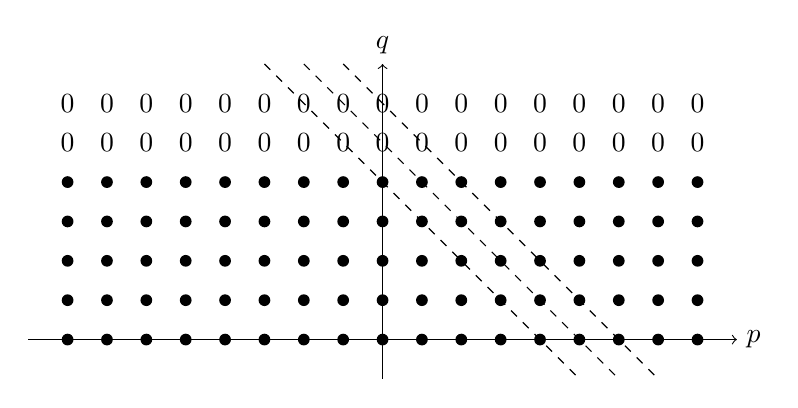
\begin{tikzpicture}[x=0.5cm, y=0.5cm]
        \draw[dashed] (-3,7) -- (5,-1);
        \draw[dashed] (-2,7) -- (6,-1);
        \draw[dashed] (-1,7) -- (7,-1);

        \draw[->] (0,-1) -- (0,7) node[above] {$q$};
        \draw[->] (-9,0) -- (9,0) node[right] {$p$};

        \foreach \p in {-8, ..., 8}
        \foreach \q in {5, ..., 6}
        \draw (\p,\q) node {$0$};

        \foreach \p in {-8, ..., 8}
        \foreach \q in {0, ..., 4}
        \draw (\p,\q) node[circle,fill,inner sep=1.5pt] {};
      \end{tikzpicture}
    \end{center}

    \noindent where all objects are \emph{finite} $2$-torsion.
  \end{proof}
\end{theorem}

For the sake of completeness and for further reference, let us look at spectral
sequences similar to the one in the last proof, but with the usual group
cohomology instead of Tate cohomology. If we replace $\widehat{H}$ with $H$,
then $H^p (G_\RR, H^q_c (X (\CC), (2\pi i)^n \, \ZZ))$ is not necessarily
$2$-torsion for $p = 0$, and the second page of the spectral sequence
\[ E_2^{pq} = H^p (G_\RR, H^q_c (X (\CC), (2\pi i)^n \, \ZZ)) \Longrightarrow
  H^{p+q}_c (G_\RR, X (\CC), (2\pi i)^n \, \ZZ) \]
looks like

\begin{center}

  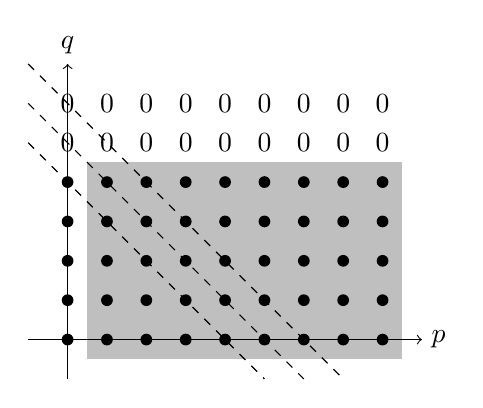
\begin{tikzpicture}[x=0.5cm, y=0.5cm]
    \fill[lightgray] (0.5,-0.5) -- (0.5,4.5) -- (8.5,4.5) -- (8.5,-0.5) -- cycle;

    \draw[dashed] (-1,5) -- (5,-1);
    \draw[dashed] (-1,6) -- (6,-1);
    \draw[dashed] (-1,7) -- (7,-1);

    \draw[->] (0,-1) -- (0,7) node[above] {$q$};
    \draw[->] (-1,0) -- (9,0) node[right] {$p$};

    \foreach \p in {0, ..., 8}
    \foreach \q in {5, ..., 6}
    \draw (\p,\q) node {$0$};

    \foreach \p in {0, ..., 8}
    \foreach \q in {0, ..., 4}
    \draw (\p,\q) node[circle,fill,inner sep=1.5pt] {};
  \end{tikzpicture}
\end{center}

\noindent where the shaded part $E_2^{pq}$, $p > 0$ consists of finitely
generated $2$-torsion groups, the line $E_2^{0q}$ consists of finitely generated
groups, and the objects $E_2^{pq}$ are zero for $q \gg 0$. It follows that the
groups $H^i (G_\RR, X (\CC), (2\pi i)^n\,\ZZ)$ are all finitely generated as
well, and they are torsion for $i \gg 0$. This is in fact $2$-torsion, and we
may see this as follows. If $P_\bullet \epi \ZZ$ is the bar-resolution of $\ZZ$
by free $\ZZ G_\RR$-modules, then the morphism of complexes

\[ \begin{tikzcd}
    \cdots\ar{r} & P_3\ar{r}\ar{d}{2} & P_2\ar{r}\ar{d}{2} & P_1\ar{r}\ar{d}{2} & P_0\ar{r}\ar{d}{2-N} & 0 \\
    \cdots\ar{r} & P_3\ar{r} & P_2\ar{r} & P_1\ar{r} & P_0\ar{r} & 0
  \end{tikzcd} \]

\begin{align*}
  \text{``}2\text{''}\colon P_\bullet & \to P_\bullet,\\
  (2-N)\colon P_0 & \to P_0,\\
  2\colon P_i & \to P_i \quad\text{for }i > 1,
\end{align*}

\noindent which induces multiplication by $2$ on $H^i (G,-)$ for $i > 0$ is
null-homotopic \cite[Theorem 6.5.8]{Weibel-94}. It is not multiplication by $2$
in degree $0$, but as the complex $R\Gamma_c (G_\RR, X (\CC), (2\pi i)^n\,\ZZ)$
is bounded, we see that it induces multiplication by $2$ on
$H^i (G_\RR, X (\CC), (2\pi i)^n\,\ZZ)$ for $i \gg 0$. So we just proved the
following.

\begin{lemma}
  \label{lemma:RGammac-GR-XC-Z-almost-perfect}
  The complex
  \[ R\Gamma_c (G_\RR, X (\CC), (2\pi i)^n\,\ZZ) =
    R\Gamma (G_\RR, R\Gamma_c (X (\CC), (2\pi i)^n\,\ZZ)) \]
    is almost perfect in the sense of \ref{dfn:almost-perfect-complex}.
\end{lemma}

As for $\QQ/\ZZ$-coefficients, we may analyze a similar spectral sequence
\[ E_2^{pq} = H^p (G_\RR, H^q_c (X (\CC), (2\pi i)^n\,\QQ/\ZZ)) \Longrightarrow
  H^{p+q} (G_\RR, X (\CC), (2\pi i)^n\,\QQ/\ZZ). \]
The second page will have groups of cofinite type on the line $E_2^{0q}$
(see \ref{thm:singular-cohomology-of-complex-varieties}) and finite $2$-torsion
groups $E_2^{pq}$ for $p > 0$. We have filtrations
\begin{multline}
  \label{eqn:ss-filtrations}
  H^{p+q} = F^0 (H^{p+q}) \supseteq
  F^1 (H^{p+q}) \supseteq
  F^2 (H^{p+q}) \supseteq \cdots\\
  \supseteq F^{p+q} (H^{p+q}) \supset F^{p+q+1} (H^{p+q}) = 0
\end{multline}
where
$$0 \to F^{p+1} (H^{p+q}) \to F^p (H^{p+q}) \to E_\infty^{pq} \to 0$$
Note that $E^{0q}_\infty$ will be groups of cofinite type, and $E^{pq}_\infty$
will be finite $2$-torsion groups for $p > 0$, as we are going to have
$$0 \to E_{r+1}^{0q} \to E_r^{0q} \to T \to 0$$
where $T$ is finite $2$-torsion, and similarly,
$$E_{r+1}^{pq} \isom \ker d_r^{pq} / \im d_r^{p-r,q+r-1}$$

\[ E_r^{p-r,q+r-1} \xrightarrow{d_r^{p-r,q+r-1}}
  E_r^{pq} \xrightarrow{d_r^{pq}}
  E_r^{p+r,q-r+1} \]

\noindent where $E_r^{pq}$ is finite $2$-torsion for $p > 0$. It follows by
induction that all the members of the filtration \eqnref{eqn:ss-filtrations} are
finite groups, except for $F^0 (H^{p+q}) = H^{p+q}$ itself, which is of cofinite
type, being an extension of a group of cofinite type $E_\infty^{0q}$ by a finite
group $F^1 (H^{p+q})$ (see \ref{lemma:extensions-of-cofinite-type-groups}).
We also see that $H^{p+q}$ is $2$-torsion for $p+q \gg 0$. This gives us the
following result.

\begin{lemma}
  \label{lemma:RGammac-GR-XC-QZ-almost-cofinite-type}
  The complex
  \[ R\Gamma_c (G_\RR, X (\CC), (2\pi i)^n\,\QQ/\ZZ) =
    R\Gamma (G_\RR, R\Gamma_c (X (\CC), (2\pi i)^n\,\QQ/\ZZ)) \]
  is almost of cofinite type in the sense of
  \ref{dfn:almost-cofinite-type-complex}.
\end{lemma}

% % % % % % % % % % % % % % % % % % % % % % % % % % % % % %

\section{Complexes
  \texorpdfstring{$R\Gamma_\text{\it fg} (X, \ZZ (n))$}{RΓ\_fg (X,Z(n))}}
\label{section:RGammafg}

\begin{definition}
  \label{definition:RGammaW}
  The morphism $\alpha_{X,n}$ in $\categ{D} (\categ{Ab})$ is given by the
  composition of morphisms
  \begin{multline*}
    \RHom (R\Gamma (X_\text{\it ét}, \ZZ^c (n)), \QQ [-2]) \to
    \RHom (R\Gamma (X_\text{\it ét}, \ZZ^c (n)), \QQ/\ZZ[-2]) \\
    \xleftarrow{\isom} R\widehat{\Gamma}_c (X_\text{\it ét}, \ZZ (n)) \to
    R\Gamma_c (X_\text{\it ét}, \ZZ (n))
  \end{multline*}

  Here the first arrow is induced by
  $\RHom (R\Gamma (X_\text{\it ét}, \ZZ^c (n)), -)$ and the canonical projection
  $\QQ \epi \QQ/\ZZ$. The second arrow is a quasi-isomorphism given by theorem
  \ref{thm:artin-verdier-duality}. The third arrow is the morphism
  \eqnref{eqn:morphism-fromRGammahatc-to-RGammac} from cohomology with compact
  support à la Milne to the usual cohomology with compact support.

  Then the complex $R\Gamma_\text{\it fg} (X, \ZZ (n))$ is defined as a cone of
  $\alpha_{X,n}$ in $\categ{D} (\categ{Ab})$:
  \begin{multline*}
    \RHom (R\Gamma (X_\text{\it ét}, \ZZ^c (n)), \QQ [-2])
    \xrightarrow{\alpha_{X,n}} R\Gamma_c (X_\text{\it ét}, \ZZ (n)) \to
    R\Gamma_\text{\it fg} (X, \ZZ (n)) \\
    \to \RHom (R\Gamma (X_\text{\it ét}, \ZZ^c (n)), \QQ [-1])
  \end{multline*}
\end{definition}

\begin{remark}
  \label{rmk:RGamma-fg-with-no-real-points}
  If $X (\RR) = \emptyset$, then
  $R\widehat{\Gamma}_c (X_\text{\it ét}, \ZZ (n))$ is the same as
  $R\Gamma_c (X_\text{\it ét}, \ZZ (n))$
  (see \ref{rmk:compact-support-a-la-Milne-with-no-real-points}), so that in
  this case we have an isomorphism of distinguished triangles
  \[ \begin{tikzcd}
      \RHom (R\Gamma (X_\text{\it ét}, \ZZ^c (n)), \QQ [-2]) \ar{r}{\idid}\ar{d} & \RHom (R\Gamma (X_\text{\it ét}, \ZZ^c (n)), \QQ [-2])\ar{d} \\
      \RHom (R\Gamma (X_\text{\it ét}, \ZZ^c (n)), \QQ/\ZZ [-2]) \ar{r}{\quiso}\ar{d} & R\Gamma_c (X_\text{\it ét}, \ZZ (n))\ar{d} \\
      \RHom (R\Gamma (X_\text{\it ét}, \ZZ^c (n)), \ZZ [-1]) \ar[dashed]{r}{\quiso}\ar{d} & R\Gamma_\text{\it fg} (X, \ZZ (n))\ar{d} \\
      \RHom (R\Gamma (X_\text{\it ét}, \ZZ^c (n)), \QQ [-1]) \ar{r}{\idid} & \RHom (R\Gamma (X_\text{\it ét}, \ZZ^c (n)), \QQ [-1])
    \end{tikzcd} \]
  where the left column is the result of application of
  $\RHom (R\Gamma (X_\text{\it ét}, \ZZ^c (n)), -)$ to an appropriate rotation
  of the triangle
  $$\ZZ \to \QQ \to \QQ/\ZZ \to \ZZ [1]$$
  We conclude that
  \[ R\Gamma_\text{\it fg} (X, \ZZ (n)) \quiso
    \RHom (R\Gamma (X_\text{\it ét}, \ZZ^c (n)), \ZZ [-1]). \]
  However, this holds only if $X (\RR) = \emptyset$. In what follows, we are not
  going to make such an assumption on $X$, even though it would save quite some
  technical work. It is still helpful to keep in mind the special case
  $X (\RR) = \emptyset$.
\end{remark}

The complex of sheaves $\ZZ^c (n)$ is bounded from below, under the assumption
that their cohomology groups are finitely generated (which is our conjecture
$\mathbf{L}^c (X_\text{\it ét}, n)$, stated in \ref{conjecture:Lc(X,n)}).

\begin{lemma}
  \label{lemma:finite-generation-implies-boundedness}
  Assuming the conjecture $\mathbf{L}^c (X_\text{\it ét}, n)$, we have
  $$H^i (X_\text{\it ét}, \ZZ^c (n)) = 0\quad\text{for }i < -2\,\dim X.$$

  \begin{proof}
    The complex of sheaves $\ZZ^c (n)$ is flat, so the short exact sequence of
    abelian groups
    $$0 \to \ZZ \to \QQ \to \QQ/\ZZ \to 0$$
    gives us a short exact sequence of étale sheaves
    $$0 \to \ZZ^c (n) \to \QQ^c (n) \to \QQ/\ZZ^c (n) \to 0$$
    and then applying $R\Gamma (X_\text{\it ét}, -)$, we obtain a distinguished
    triangle in $\categ{D} (\categ{Ab})$
    \[ R\Gamma (X_\text{\it ét}, \ZZ^c (n)) \to
      R\Gamma (X_\text{\it ét}, \QQ^c (n)) \to
      R\Gamma (X_\text{\it ét}, \QQ/\ZZ^c (n)) \to
      R\Gamma (X_\text{\it ét}, \ZZ^c (n)) [1] \]
    Now according to \cite[Lemma 5.12]{Morin-14} (note that the proof there also
    uses Geisser's duality), we have
    \[ H^i (X_\text{\it ét}, \QQ/\ZZ^c (n)) = 0
      \quad\text{for }i < -2\,\dim X, \]
    and the above triangle implies that
    \[ H^i (X_\text{\it ét}, \QQ^c (n)) \isom
      H^i (X_\text{\it ét}, \ZZ^c (n))
      \quad\text{for }i < -2\,\dim X. \]
    However, $H^i (X_\text{\it ét}, \QQ^c (n))$ is a $\QQ$-vector space, and
    according to the conjecture $\mathbf{L}^c (X_\text{\it ét}, n)$, the groups
    $H^i (X_\text{\it ét}, \ZZ^c (n))$ are finitely generated over $\ZZ$.
    This means that for $i < -2\,\dim X$ these groups are trivial.
  \end{proof}
\end{lemma}

\begin{proposition}
  \label{prop:RGammafg-almost-perfect}
  The complex $R\Gamma_\text{\it fg} (X, \ZZ (n))$ is almost perfect in the
  sense of \ref{dfn:almost-perfect-complex}, i.e. its cohomology groups
  $H^i_\text{\it fg} (X, \ZZ (n)) \dfn H^i (R\Gamma_\text{\it fg} (X, \ZZ (n)))$
  are finitely generated, trivial for $i \ll 0$, and only have $2$-torsion for
  $i \gg 0$.

  \begin{proof}
    By the definition of $R\Gamma_\text{\it fg} (X, \ZZ (n))$, we have a long
    exact sequence in cohomology
    \[ \begin{tikzcd}[column sep=1em,font=\small]
        \cdots\ar{r} & \Hom (H^{2-i} (X_\text{\it ét}, \ZZ^c (n)), \QQ) \ar{r}{H^i (\alpha_{X,n})} &[2em] H^i_c (X_\text{\it ét}, \ZZ (n))\ar{r}\ar[draw=none]{d}[name=X, anchor=center]{} & H^i_\text{\it fg} (X, \ZZ (n)) \ar[rounded corners,to path={ -- ([xshift=2ex]\tikztostart.east) |- (X.center) \tikztonodes -| ([xshift=-2ex]\tikztotarget.west) -- (\tikztotarget)}]{dll}[at end]{\delta^i} \\
        & \Hom (H^{1-i} (X_\text{\it ét}, \ZZ^c (n)), \QQ)\ar{r}{H^{i+1} (\alpha_{X,n})} & H^{i+1}_c (X_\text{\it ét}, \ZZ (n))\ar{r} & \cdots
      \end{tikzcd} \]

    We consider short exact sequences
    \[ \begin{tikzcd}[row sep=0.5em]
        0 \ar{r} & \ker \delta^i \ar{r}\ar[equals]{d} & H^i_\text{\it fg} (X, \ZZ (n)) \ar{r} & \im \delta^i \ar{r}\ar[equals]{d} & 0\\
        & \coker H^i (\alpha_{X,n}) & & \ker H^{i+1} (\alpha_{X,n})
      \end{tikzcd} \]

    By the definition of $\alpha_{X,n}$, the morphism $H^i (\alpha_{X,n})$
    factors as
    \begin{multline*}
      \Hom (H^{2-i} (X_\text{\it ét}, \ZZ^c (n)), \QQ) \to
      \Hom (H^{2-i} (X_\text{\it ét}, \ZZ^c (n)), \QQ/\ZZ) \\
      \xrightarrow{\isom} \widehat{H}^i_c (X_\text{\it ét}, \ZZ (n)) \to
      H^i_c (X_\text{\it ét}, \ZZ (n))
    \end{multline*}

    Here the morphism
    $\widehat{H}^i_c (X_\text{\it ét}, \ZZ (n)) \to H^i_c (X_\text{\it ét}, \ZZ (n))$
    is identity, except for some \emph{finite} $2$-torsion. Indeed, this
    morphism sits in the long exact sequence \eqnref{eqn:Hc-hat-vs-Hc-les}:
    \begin{multline*}
      \cdots \to \widehat{H}^{i-1} (G_\RR, (Rf_! \ZZ (n))_\CC) \to
      \widehat{H}^i_c (X_\text{\it ét}, \ZZ (n)) \to
      H^i_c (X_\text{\it ét}, \ZZ (n)) \\
      \to \widehat{H}^i (G_\RR, (Rf_! \ZZ (n))_\CC) \to \cdots
    \end{multline*}
    and $\widehat{H}^i (G_\RR, (Rf_! \ZZ (n))_\CC)$ is finite $2$-torsion
    according to \ref{thm:RGammahat-GR-Rf!ZnC}.

    The group $H^{2-i} (X_\text{\it ét}, \ZZ^c (n))$ is finitely generated
    according to the conjecture $\mathbf{L}^c (X_\text{\it ét}, n)$
    (see \ref{conjecture:Lc(X,n)}). If this group is of the form
    $\ZZ^{\oplus r}\oplus T$, the morphism $H^i (\alpha_{X,n})$ is given by
    \[ \QQ^{\oplus r} \epi (\QQ/\ZZ)^{\oplus r} \mono
      \widehat{H}^i_c (X_\text{\it ét}, \ZZ (n)) \to
      H^i_c (X_\text{\it ét}, \ZZ (n)) \]
    where
    $(\QQ/\ZZ)^{\oplus r} \mono \widehat{H}^i_c (X_\text{\it ét}, \ZZ (n))$
    is the inclusion of the maximal divisible subgroup in the group of cofinite
    type
    \[ \widehat{H}^i_c (X_\text{\it ét}, \ZZ (n)) \isom
      \Hom (H^{2-i} (X_\text{\it ét}, \ZZ^c (n)), \QQ/\ZZ). \]
    Both kernel and cokernel of the above map are finitely generated, hence
    $H^i_\text{\it fg} (X, \ZZ (n))$ is finitely generated.

    As we observed in \ref{lemma:finite-generation-implies-boundedness}, again
    assuming the conjecture $\mathbf{L}^c (X_\text{\it ét}, n)$, we may deduce
    that the complex $\ZZ^c (n)$ is bounded from below. This means that for
    $i \ll 0$ we have
    \[ \ker H^{i+1} (\alpha_{X,n}) = 0,
      \quad H^i_\text{\it fg} (X, \ZZ (n)) \isom
      \coker H^i (\alpha_{X,n}) = H^i_c (X_\text{\it ét}, \ZZ (n)). \]
    For $i < 1$ we have $H^i_c (X_\text{\it ét}, \ZZ (n)) = 0$, and for
    $i \gg 0$ we know that
    \[ \widehat{H}^i_c (X_\text{\it ét}, \ZZ (n)) \isom
      \Hom (H^{2-i} (X_\text{\it ét}, \ZZ^c (n)), \QQ/\ZZ) = 0, \]
    again by boundedness of $\ZZ^c (n)$ from below. The only difference between
    $H^i_c (X_\text{\it ét}, \ZZ (n))$ and
    $\widehat{H}^i_c (X_\text{\it ét}, \ZZ (n))$ is some finite $2$-torsion.
  \end{proof}
\end{proposition}

\begin{observation}
  \label{obs:RGammafg-defined-up-to-unique-iso}
  $R\Gamma_\text{\it fg} (X, \ZZ (n))$ is defined up to a unique isomorphism in
  $\categ{D} (\categ{Ab})$.

  \begin{proof}
    The complex $\RHom (R\Gamma (X_\text{\it ét}, \ZZ^c (n)), \QQ [-2])$
    consists of $\QQ$-vector spaces, and $R\Gamma_\text{\it fg} (X, \ZZ (n))$ is
    almost perfect, so we are in the situation of \ref{TR3-TR1-with-uniqueness}.
  \end{proof}
\end{observation}

\begin{observation}
  \label{RGammafg-with-Q-and-Z/nZ-coeffs}
  Fix a distinguished triangle defining $R\Gamma_\text{\it fg} (X, \ZZ (n))$:
  \begin{multline*}
    \RHom (R\Gamma (X_\text{\it ét}, \ZZ^c (n)), \QQ [-2])
    \xrightarrow{\alpha_{X,n}} R\Gamma_c (X_\text{\it ét}, \ZZ (n))
    \xrightarrow{f} R\Gamma_\text{\it fg} (X, \ZZ (n)) \\
    \xrightarrow{g} \RHom (R\Gamma (X_\text{\it ét}, \ZZ^c (n)), \QQ [-1])
  \end{multline*}

  \begin{enumerate}
  \item[1)] For each $m = 1,2,3,\ldots$ the morphism
    \[ f \otimes \ZZ/m\ZZ \colon
      R\Gamma_c (X_\text{\it ét}, \ZZ (n)) \otimes_\ZZ^\mathbf{L} \ZZ/m\ZZ
      \xrightarrow{\isom}
      R\Gamma_\text{\it fg} (X, \ZZ (n)) \otimes_\ZZ^\mathbf{L} \ZZ/m\ZZ \]
    is iso. Further, we have
    \begin{multline*}
      R\Gamma_c (X_\text{\it ét}, \ZZ (n)) \otimes_\ZZ^\mathbf{L} \ZZ/m\ZZ \isom
      R\Gamma_c (X_\text{\it ét}, \ZZ/m\ZZ (n)) \\
      \dfn R\Gamma_c (X_\text{\it ét}, \ZZ (n) \otimes^\mathbf{L} \ZZ/m\ZZ).
    \end{multline*}

  \item[2)] The morphism
    \[ g\otimes\QQ \colon
      R\Gamma_\text{\it fg} (X, \ZZ (n)) \otimes_\ZZ \QQ \xrightarrow{\isom}
      \RHom (R\Gamma (X_\text{\it ét}, \ZZ^c (n)), \QQ [-1]) \]
    is iso.
  \end{enumerate}

  \begin{proof}
    The statement 1) follows from the fact that the complexes
    $$\RHom (R\Gamma (X_\text{\it ét}, \ZZ^c (n)), \QQ [\ldots])$$
    consist of $\QQ$-vector spaces, and thus
    \begin{multline*}
      \RHom (R\Gamma (X_\text{\it ét}, \ZZ^c (n)), \QQ [\ldots]) \otimes_\ZZ^\mathbf{L} \ZZ/m\ZZ \\
      \quiso \RHom (R\Gamma (X_\text{\it ét}, \ZZ^c (n)), \QQ [\ldots]) \otimes_\ZZ \ZZ/m\ZZ \quiso 0.
    \end{multline*}
    Next, 2) follows from the fact that the cohomology of the étale sheaf
    $\ZZ (n)$ is torsion, and therefore
    \begin{align*}
      H^i (R\Gamma_c (X_\text{\it ét}, \ZZ (n)) \otimes_\ZZ \QQ) & \isom H^i_c (X_\text{\it ét}, \ZZ (n)) \otimes_\ZZ \QQ = 0,\\
      R\Gamma_c (X_\text{\it ét}, \ZZ (n)) \otimes_\ZZ \QQ & \quiso 0.
    \end{align*}

  \end{proof}
\end{observation}



% % % % % % % % % % % % % % % % % % % % % % % % % % % % % %

\section{Complexes
  \texorpdfstring{$R\Gamma_\text{\it W,c} (X, \ZZ (n))$}{RΓ\_W,c (X,Z(n))}}
\label{section:RGammaWc}

To define complexes $R\Gamma_\text{\it W,c} (X, \ZZ (n))$, we first construct a
morphism
\[ i_\infty^*\colon
  R\Gamma_\text{\it fg} (X, \ZZ (n)) \to
  R\Gamma_c (G_\RR, X (\CC), (2\pi i)^n\,\ZZ). \]
By definition, it sits in the morphism of distinguished triangles
\begin{equation}
  \label{eqn:triangle-defining-i-infty}
  \begin{tikzcd}
    \RHom (R\Gamma (X, \ZZ^c (n)), \QQ [-2]) \ar{d}[swap]{\alpha_{X,n}}\ar{r} & 0\ar{d} \\
    R\Gamma_c (X_\text{\it ét}, \ZZ (n)) \ar{r}{u_\infty^*}\ar{d} &  R\Gamma_c (G_\RR, X (\CC), (2\pi i)^n\,\ZZ) \ar{d}{\idid} \\
    R\Gamma_\text{\it fg} (X, \ZZ (n)) \ar[dashed]{r}{i_\infty^*}\ar{d} & R\Gamma_c (G_\RR, X (\CC), (2\pi i)^n\,\ZZ) \ar{d} \\
    \RHom (R\Gamma (X, \ZZ^c (n)), \QQ [-1])\ar{r} & 0 \\
  \end{tikzcd}
\end{equation}

Here
\[ u_\infty^*\colon
  R\Gamma (X_\text{\it ét}, \ZZ (n)) \to
  R\Gamma_c (G_\RR, X (\CC), (2\pi i)^n\,\ZZ) \]
is some morphism, to be defined below, such that the composition
$u_\infty^*\circ \alpha_{X,n}$ is zero. Then by the axiom (TR3) there exists
some morphism $i_\infty^*$. The fact that $u_\infty^*\circ \alpha_{X,n} = 0$
will be a delicate issue, which is the main goal of this section. However, once
we know that, $i_\infty^*$ is automatically unique.

\begin{observation}
  \label{obs:uniqueness-of-i-infty}
  If $i_\infty^*$ exists, then it is unique.
\end{observation}

\begin{proof}[Proof of \ref{obs:uniqueness-of-i-infty}]
  We may apply \ref{TR3-TR1-with-uniqueness}, because
  $\RHom (R\Gamma (X, \ZZ^c (n)), \QQ [-2])$ is a complex of $\QQ$-vector spaces
  and both
  \[ R\Gamma_\text{\it fg} (X, \ZZ (n))
    \quad\text{and}\quad
    R\Gamma_c (G_\RR, X (\CC), (2\pi i)^n\,\ZZ) \]
  are almost perfect complexes by \ref{prop:RGammafg-almost-perfect} and
  \ref{lemma:RGammac-GR-XC-Z-almost-perfect}.
\end{proof}

\begin{proposition}
  \label{propn:image-of-QZn-under-alpha}
  Consider the morphism
  \[ \alpha^*\colon \categ{Sh} (X_\text{\it ét}) \to
    \categ{Sh} (G_\RR, X (\CC)), \]
  as described in \S\ref{section:etale-and-equivariant-sheaves}. For the sheaf
  $$\QQ/\ZZ (n) \dfn \bigoplus_p \dirlim_r  j_{p!} \mu_{p^r}^{\otimes n}$$
  defined in \S\ref{section:cycle-complex-for-negative-n} we have an isomorphism
  of $G_\RR$-equivariant constant sheaves on $X (\CC)$
  \[ \alpha^* \QQ/\ZZ (n) \isom
    \frac{(2\pi i)^n\,\QQ}{(2\pi i)^n\,\ZZ}
    \rdfn (2\pi i)^n\,\QQ/\ZZ. \]

  \begin{proof}
    First of all, since $\alpha^*$ is the composition of certain inverse image
    functors $\gamma^*$ and $\epsilon^*$ (which are left adjoint) and an
    equivalence of categories $\delta_*$, the functor $\alpha^*$ preserves
    colimits, and in particular
    \begin{equation}
      \label{eqn:alpha-star-commutes-with-colimits}
      \alpha^* \QQ/\ZZ (n) \isom
      \bigoplus_p \dirlim_r \alpha^* j_{p!} \mu_{p^r}^{\otimes n}.
    \end{equation}

    Another formal observation is that the base change from $\Spec \ZZ$ to
    $\Spec \CC$ factors through the base change to $\Spec \ZZ [1/p]$, and then
    $j_p^* \circ j_{p!} = \id{\categ{Sh} (X [1/p]_\text{\it ét})}$:

    \[ \begin{tikzcd}
        \categ{Sh} (X [1/p]_\text{\it ét}) \ar{r}{j_{p!}}\ar{drr}[swap]{\idid} & \categ{Sh} (X_\text{\it ét}) \ar{rr}{\gamma^*}\ar{dr}{j_p^*} & & \categ{Sh} (X_{\CC,\text{\it ét}}) \\
        & & \categ{Sh} (X [1/p]_\text{\it ét})\ar[dashed]{ur}
      \end{tikzcd} \]

    \noindent which means that we may safely erase ``$j_{p!}$'' in
    \eqnref{eqn:alpha-star-commutes-with-colimits}, and everything boils down to
    calculating the sheaves
    \[ \alpha^* \mu_{p^r}^{\otimes n} =
      \alpha^* \iHom_{X [1/p]} (\mu_{p^r}^{\otimes (-n)}, \ZZ/p^r \ZZ). \]
    As we base change to $\Spec \CC$, the étale sheaf $\mu_{p^r}$ simply becomes
    the constant sheaf $\mu_{p^r} (\CC)$ on $X (\CC)$, and
    \[ \alpha^* \mu_{p^r}^{\otimes n} =
      \iHom_{X (\CC)} (\mu_{p^r}^{\otimes (-n)} (\CC), \ZZ/p^r \ZZ). \]
    In \ref{lemma:all-roots-of-unity-as-QZ} we calculated the colimit of such
    things to be $(2\pi i)^n\,\QQ/\ZZ$.
  \end{proof}
\end{proposition}

\begin{definition}
  \label{dfn:u-infty}
  The morphism
  \[ u_\infty^*\colon R\Gamma_c (X_\text{\it ét}, \ZZ(n)) \to
    R\Gamma_c (G_\RR, X (\CC), (2\pi i)^n\,\ZZ) \]
  is given by the composition
  \begin{multline*}
    R\Gamma_c (X_\text{\it ét}, \ZZ(n)) \dfn
    R\Gamma_c (X_\text{\it ét}, \QQ/\ZZ (n)) [-1]\\
    \xrightarrow{v_\infty^* [-1]}
    R\Gamma_c (G_\RR, X (\CC), (2\pi i)^n\,\QQ/\ZZ) [-1] \to
    R\Gamma_c (G_\RR, X (\CC), (2\pi i)^n\,\ZZ)
  \end{multline*}

  \noindent Here the last arrow is induced by
  $(2\pi i)^n\,\QQ/\ZZ [-1] \to (2\pi i)^n\,\ZZ$, which comes from the
  distinguished triangle of constant $G_\RR$-equivariant sheaves
  \[ (2\pi i)^n\,\ZZ \to
    (2\pi i)^n\,\QQ \to
    (2\pi i)^n\,\QQ/\ZZ \to
    (2\pi i)^n\,\ZZ [1] \]
  and the arrow
  \[ v_\infty^*\colon R\Gamma_c (X_\text{\it ét}, \QQ/\ZZ (n)) \to
    R\Gamma_c (G_\RR, X (\CC), (2\pi i)^n\,\QQ/\ZZ) \]
  is induced by the morphism
  \[ \Gamma_c (X_\text{\it ét}, \QQ/\ZZ (n)) \to
    \Gamma_c (G_\RR, X (\CC), \alpha^* \QQ/\ZZ (n)) \isom
    \Gamma_c (G_\RR, X (\CC), (2\pi i)^n\,\QQ/\ZZ) \]
  (see \ref{prop:inverse-image-gamma} and \ref{propn:image-of-QZn-under-alpha}).
\end{definition}

\begin{theorem}
  \label{thm:u-alpha-0}
  For any arithmetic scheme $X$ one has $u_\infty^* \circ \alpha_{X,n} = 0$ in
  the derived category.
\end{theorem}

This seems to be rather nontrivial; our proof will be based on the following
result about $\ell$-adic cohomology.

\begin{proposition}
  \label{prop:l-adic-cohomology-key-lemma}
  Let $f\colon X\to \Spec \ZZ$ be an arithmetic scheme (that is, with $f$
  separated, of finite type). Let $n < 0$. Then for any prime $\ell$ we have
  $$(H^i_c (X_{\overline{\QQ},\text{\it ét}}, \QQ_\ell/\ZZ_\ell (n))^{G_\QQ})_{div} = 0.$$

  \begin{proof}
    Let us recall some facts about $\ell$-adic cohomology. We refer to
    \cite[Exposé VI]{SGA5} for details. Let us first consider the sheaf
    $\ZZ_\ell (n)$. It is a \term{constructible $\ZZ_\ell$-sheaf}\footnote{Or
      simply \term{$\ZZ_\ell$-sheaf} in the terminology of
      \cite[Rapport]{SGA4-1-2}.} on $X$ in the sense of
    \cite[Exposé VI, 1.1.1]{SGA5}. We would like to compare the cohomology of
    $\ZZ_\ell (n)$ on $X_{\overline{\QQ},\text{\it ét}}$ and
    $X_{\overline{\FF_p},\text{\it ét}}$, where $p$ is some prime different from
    $\ell$, to be determined later.  For this we fix some algebraic closures
    $\overline{\QQ}/\QQ$ and $\overline{\FF_p}/\FF_p$ and consider the
    corresponding morphisms
    \[ \overline{\eta}\colon \Spec \overline{\QQ} \to \Spec \ZZ, \quad
      \overline{x}\colon \Spec \overline{\FF_p} \to \Spec \ZZ. \]
    Let $X_{\overline{\QQ},\text{\it ét}}$ and
    $X_{\overline{\FF_p},\text{\it ét}}$ be the pullbacks of $X$ along the above
    morphisms:

    \[ \begin{tikzcd}
        X_{\overline{\QQ}} \ar{r}\tikzpb\ar{d}[swap]{f_{\overline{\QQ}}} & X \ar{d}{f} & X_{\overline{\FF_p}} \ar{l}\ar{d}{f_{\overline{\FF_p}}}\tikzpbur \\
        \Spec \overline{\QQ} \ar{r}[swap]{\overline{\eta}} & \Spec \ZZ & \Spec \overline{\FF_p} \ar{l}{\overline{x}}
      \end{tikzcd} \]

    According to \cite[Exposé VI, 2.2.3]{SGA5}, the proper base change theorem
    holds for constructible $\ZZ_\ell$-sheaves. It gives us isomorphisms
    \[ H^i_c (X_{\overline{\QQ}, \text{\it ét}}, \ZZ_\ell (n)) \isom
      (R^i f_! \ZZ_\ell (n))_{\overline{\eta}},
      \quad
      H^i_c (X_{\overline{\FF_p}, \text{\it ét}}, \ZZ_\ell (n)) \isom
      (R^i f_! \ZZ_\ell (n))_{\overline{x}}, \]
    where $R^i f_! \ZZ_\ell (n)$ is the same sheaf on $\Spec \ZZ$, and we take
    its different stalks to get cohomology with compact support on different
    fibers. The construction of higher direct images with proper support
    $R^i f_! \mathcal{F}$ for $\ell$-adic sheaves is given in
    \cite[Exposé VI, \S 2.2]{SGA5}. The key nontrivial fact that we need is that
    for every morphism (of locally noetherian schemes) $f\colon X\to Y$,
    separated of finite type, if $\mathcal{F}$ is a constructible
    $\ZZ_\ell$-sheaf on $X$, then $R^i f_! \mathcal{F}$ is a constructible
    $\ZZ_\ell$-sheaf on $Y$.

    According to \cite[Exposé VI, 1.2.6]{SGA5}, for a projective system of
    abelian sheaves $\mathcal{F} = (\mathcal{F}_n)_{n\in\NN}$ on
    $X_\text{\it ét}$, the following are equivalent:

    \begin{enumerate}
    \item[1)] $\mathcal{F}$ is a constructible $\ZZ_\ell$-sheaf,

    \item[2)] every open subscheme $U\subset X$ is a finite union of locally
      closed pieces $Z_i$ where $\left.\mathcal{F}\right|_{Z_i}$ is a
      \term{twisted constant constructible $\ZZ_\ell$-sheaf}\footnote{A
        \term{faisceau lisse} in the terminology of \cite[Rapport]{SGA4-1-2}.}.
    \end{enumerate}

    Being ``twisted constant'' means that each sheaf $\mathcal{F}_n$ in the
    projective system $(\mathcal{F}_n)_{n\in\NN}$ is locally constant.
    The importance of twisted constant sheaves is explained by the following
    property \cite[Exposé VI, 1.2.4, 1.2.5]{SGA5}: for a connected locally
    noetherian scheme $X$, the category of twisted constant
    $\ZZ_\ell$-constructible sheaves on $X$ is equivalent to the category of
    finitely generated $\ZZ_\ell$-modules with a continuous action of the étale
    fundamental group $\pi_1^\text{\it ét} (X)$.

    In our setting, all this means that there exists an open subscheme
    $$U = \Spec \ZZ_S \subset \Spec \ZZ,$$
    where $\ZZ_S$ denotes the localization of $\ZZ$ at a finite set of primes
    $S$, such that the sheaves $R^i f_! \ZZ_\ell (n)$ are twisted constant on
    $U$.  By removing all the necessary bad primes, we can make sure this holds
    for all $i$.

    Now according to \cite[Book IX, Proposition 20]{Elements}, there exists some
    prime $p \notin S$ (that is, $(p) \in U$), for which we may consider the
    following picture:
    \[ \begin{tikzcd}
        X_{\overline{\QQ}} \ar{r}\tikzpb\ar{d}[swap]{f_{\overline{\QQ}}} & X_U \ar{d}{f_U} & X_{\overline{\FF_p}} \ar{l}\ar{d}{f_{\overline{\FF_p}}}\tikzpbur \\
        \Spec \overline{\QQ} \ar{r}[swap]{\overline{\eta}} & U & \Spec \overline{\FF_p} \ar{l}{\overline{x}}
      \end{tikzcd} \]

    It follows that we have isomorphisms
    \begin{equation}
      \label{eqn:iso-pbc-Zl-Gal(QS/Q)}
      H^i_c (X_{\overline{\QQ}, \text{\it ét}}, \ZZ_\ell (n)) \isom
      (R^i f_{U,!} \ZZ_\ell (n))_{\overline{\eta}} \isom
      (R^i f_{U,!} \ZZ_\ell (n))_{\overline{x}} \isom
      H^i_c (X_{\overline{\FF_p}, \text{\it ét}}, \ZZ_\ell (n)),
    \end{equation}

    \noindent of finitely generated $\ZZ_\ell$-modules with continuous action of
    $$\pi_1^\text{\it ét} (U) \isom \Gal (\QQ_S/\QQ),$$
    where $\QQ_S/\QQ$ denotes a maximal extension of $\QQ$ unramified outside of
    $S$. We note that $(R^i f_{U,!} \ZZ_\ell (n))_{\overline{\eta}}$ naturally
    carries an action of $\pi_1^\text{\it ét} (U, \overline{\eta})$, while
    $(R^i f_{U,!} \ZZ_\ell (n))_{\overline{x}}$ carries an action of
    $\pi_1^\text{\it ét} (U, \overline{x})$, and the isomorphism in the middle
    of \eqnref{eqn:iso-pbc-Zl-Gal(QS/Q)} sweeps under the rug an identification
    of $\pi_1^\text{\it ét} (U, \overline{\eta})$ with
    $\pi_1^\text{\it ét} (U, \overline{x})$.

    To state this more accurately, note that the $\ZZ_\ell$-module
    $H^i_c (X_{\overline{\QQ}, \text{\it ét}}, \ZZ_\ell (n))$ carries a natural
    action of $G_\QQ$ while
    $H^i_c (X_{\overline{\FF_p}, \text{\it ét}}, \ZZ_\ell (n))$ carries a
    natural action of $G_{\FF_p}$. After making the necessary choices, we have
    $G_{\QQ_p} \subset G_\QQ$ and a short exact sequence
    $$1 \to I_p \to G_{\QQ_p} \to G_{\FF_p} \to 1$$
    where $I_p$ is the inertia subgroup, acting trivially on
    $H^i_c (X_{\overline{\QQ}, \text{\it ét}}, \ZZ_\ell (n))$. We have thus
    isomorphisms of finitely generated $\ZZ_\ell$-modules
    \[ H^i_c (X_{\overline{\QQ}, \text{\it ét}}, \ZZ_\ell (n)) \isom
      H^i_c (X_{\overline{\FF_p}, \text{\it ét}}, \ZZ_\ell (n)), \]
    equivariant under the action of $G_{\QQ_p}/I_p$ on the left hand side and of
    $G_{\FF_p}$ on the right hand side. To relate all this to $\QQ_\ell (n)$ and
    $\QQ_\ell/\ZZ_\ell (n)$-coefficients, note that we have the following
    isomorphic long exact sequences in cohomology
    \begin{equation}
      \label{eqn:Zl-Ql-Ql/Zl-les}
      \begin{tikzcd}[column sep=small, font=\small]
        \vdots \ar{d} & \vdots \ar{d} \\
        H_c^{i-1} (X_{\overline{\QQ},\text{\it ét}}, \QQ_\ell/\ZZ_\ell (n)) \ar{d}{\delta}\ar{r}{\isom} & H_c^{i-1} (X_{\overline{\FF_p},\text{\it ét}}, \QQ_\ell/\ZZ_\ell (n))  \ar{d}{\delta} \\
        H_c^i (X_{\overline{\QQ},\text{\it ét}}, \ZZ_\ell (n)) \ar{d}{\phi}\ar{r}{\isom} & H_c^i (X_{\overline{\FF_p},\text{\it ét}}, \ZZ_\ell (n)) \ar{d}{\phi} \\
        H_c^i (X_{\overline{\QQ},\text{\it ét}}, \QQ_\ell (n)) \ar{d}{\psi}\ar{r}{\isom} & H_c^i (X_{\overline{\FF_p},\text{\it ét}}, \QQ_\ell (n)) \ar{d}{\psi} \\
        H_c^i (X_{\overline{\QQ},\text{\it ét}}, \QQ_\ell/\ZZ_\ell (n)) \ar{r}\ar{d}{\isom} & H_c^i (X_{\overline{\FF_p},\text{\it ét}}, \QQ_\ell/\ZZ_\ell (n)) \ar{d} \\
        \vdots & \vdots \\
      \end{tikzcd}
    \end{equation}

    Here
    \begin{align*}
      H_c^i (X_{\overline{\QQ},\text{\it ét}}, \QQ_\ell (n)) & = H_c^i (X_{\overline{\QQ},\text{\it ét}}, \ZZ_\ell (n))\otimes_{\ZZ_\ell} \QQ_\ell,\\
      H_c^i (X_{\overline{\FF_p},\text{\it ét}}, \QQ_\ell (n)) & = H_c^i (X_{\overline{\FF_p},\text{\it ét}}, \ZZ_\ell (n))\otimes_{\ZZ_\ell} \QQ_\ell,
    \end{align*}
    and the arrows $\phi$ above are canonical localization morphisms.
    The horizontal arrows are equivariant isomorphisms in the above sense.
    Note that we have
    \begin{multline*}
      H^i_c (X_{\overline{\QQ}, \text{\it ét}}, \QQ_\ell/\ZZ_\ell (n))^{G_\QQ} \mono
      H^i_c (X_{\overline{\QQ}, \text{\it ét}}, \QQ_\ell/\ZZ_\ell (n))^{G_{\QQ_p}/I_p} \\
      \isom H^i_c (X_{\overline{\FF_p}, \text{\it ét}}, \QQ_\ell/\ZZ_\ell (n))^{G_{\FF_p}},
    \end{multline*}
    so in order to prove that
    $$(H^i_c (X_{\overline{\QQ},\text{\it ét}}, \QQ_\ell/\ZZ_\ell (n))^{G_\QQ})_{div} = 0,$$
    it will be enough to show that
    $$(H^i_c (X_{\overline{\FF_p},\text{\it ét}}, \QQ_\ell/\ZZ_\ell (n))^{G_{\FF_p}})_{div} = 0.$$
    From now on we move to the characteristic $p$ and consider the fixed points
    of $G_{\FF_p}$ acting on the $\ZZ_\ell$-module
    $H^i_c (X_{\overline{\FF_p},\text{\it ét}}, \QQ_\ell/\ZZ_\ell (n))$. In the
    long exact sequence \eqnref{eqn:Zl-Ql-Ql/Zl-les}, we have (keeping in mind
    that $\phi$ is merely the localization morphism):
    \begin{align*}
      \ker \phi & = H^i_c (X_{\overline{\FF_p},\text{\it ét}}, \ZZ_\ell (n))_{tor},\\
      \ker \psi & = \im \phi \isom H^i_c (X_{\overline{\FF_p},\text{\it ét}}, \ZZ_\ell (n)) / \ker \phi \\
                & \quad\quad\quad = \frac{H^i_c (X_{\overline{\FF_p},\text{\it ét}}, \ZZ_\ell (n))}{H^i_c (X_{\overline{\FF_p},\text{\it ét}}, \ZZ_\ell (n))_{tor}} \rdfn H^i_c (X_{\overline{\FF_p},\text{\it ét}}, \ZZ_\ell (n))_{cotor},\\
      \im \psi & = H_c^i (X_{\overline{\FF_p},\text{\it ét}}, \QQ_\ell/\ZZ_\ell (n))_{div}.
    \end{align*}

    This gives us a short exact sequence
    \begin{multline*}
      0 \to H^i_c (X_{\overline{\FF_p},\text{\it ét}}, \ZZ_\ell (n))_{cotor} \to
      H^i_c (X_{\overline{\FF_p},\text{\it ét}}, \QQ_\ell (n)) \\
      \to H^i_c (X_{\overline{\FF_p},\text{\it ét}}, \QQ_\ell/\ZZ_\ell (n))_{div} \to 0
    \end{multline*}
    After taking the $G_{\FF_p}$-invariants, we obtain a long exact sequence of
    cohomology groups
    \begin{multline}
      \label{eqn:cohomology-long-exact-sequence-with-GFp}
      0 \to (H^i_c (X_{\overline{\FF_p},\text{\it ét}}, \ZZ_\ell (n))_{cotor})^{G_{\FF_p}} \to
      H^i_c (X_{\overline{\FF_p},\text{\it ét}}, \QQ_\ell (n))^{G_{\FF_p}} \\
      \to (H^i_c (X_{\overline{\FF_p},\text{\it ét}}, \QQ_\ell/\ZZ_\ell (n))_{div})^{G_{\FF_p}} \to
      H^1 (G_{\FF_p}, H^i_c (X_{\overline{\FF_p},\text{\it ét}}, \ZZ_\ell (n))_{cotor}) \to \cdots
    \end{multline}

    We claim that
    \begin{equation}
      \label{eqn:SGA-7-expose-XXI-5-5-3}
      H^i_c (X_{\overline{\FF_p},\text{\it ét}}, \QQ_\ell (n))^{G_{\FF_p}} = 0.
    \end{equation}

    Indeed, according to \cite[Exposé XXI, 5.5.3]{SGA7}, the eigenvalues of the
    geometric Frobenius acting on
    $H^i_c (X_{\overline{\FF_p},\text{\it ét}}, \QQ_\ell)$ are algebraic
    integers. We are twisting $\QQ_\ell$ by $n$, so the eigenvalues of Frobenius
    lie in $p^{-n}\,\overline{\ZZ}$. Since $n < 0$ by our assumption, this
    implies that $1$ does not occur as an eigenvalue.

    Now \eqnref{eqn:SGA-7-expose-XXI-5-5-3} and the long exact sequence
    \eqnref{eqn:cohomology-long-exact-sequence-with-GFp} imply that there is a
    monomorphism
    \[ (H^i_c (X_{\overline{\FF_p},\text{\it ét}}, \QQ_\ell/\ZZ_\ell (n))_{div})^{G_{\FF_p}} \mono
      H^1 (G_{\FF_p}, H^i_c (X_{\overline{\FF_p},\text{\it ét}}, \ZZ_\ell (n))_{cotor}), \]
    which restricts to a monomorphism between the maximal divisible subgroups
    \[ ((H^i_c (X_{\overline{\FF_p},\text{\it ét}}, \QQ_\ell/\ZZ_\ell (n))_{div})^{G_{\FF_p}})_{div} \mono
      H^1 (G_{\FF_p}, H^i_c (X_{\overline{\FF_p},\text{\it ét}}, \ZZ_\ell (n))_{cotor})_{div}. \]
    However,
    $H^1 (G_{\FF_p}, H^i_c (X_{\overline{\FF_p},\text{\it ét}}, \ZZ_\ell (n))_{cotor})$
    is a finitely generated $\ZZ_\ell$-module, and therefore its maximal
    divisible subgroup is trivial. We have therefore
    \[ (H^i_c (X_{\overline{\FF_p},\text{\it ét}}, \QQ_\ell/\ZZ_\ell (n))^{G_{\FF_p}})_{div} =
      ((H^i_c (X_{\overline{\FF_p},\text{\it ét}}, \QQ_\ell/\ZZ_\ell (n))_{div})^{G_{\FF_p}})_{div} = 0. \]
    (For the first equality, note that for any $G$-module $A$ one has
    $((A_{div})^G)_{div} = (A^G)_{div}$.)
  \end{proof}
\end{proposition}

\begin{proof}[Now we are ready to prove \ref{thm:u-alpha-0}]
  The morphism $\alpha_{X,n}$ is defined on
  $$\RHom (R\Gamma (X_\text{\it ét}, \ZZ^c (n)), \QQ [-2]),$$
  which is a complex of $\QQ$-vector spaces, so it will be enough to show that
  $v_\infty^*$ is a torsion element in the abelian group
  $$\Hom_{\categ{D} (\categ{Ab})} (R\Gamma_c (X_\text{\it ét}, \QQ/\ZZ (n)), \, R\Gamma_c (G_\RR, X (\CC), (2\pi i)^n\,\QQ/\ZZ)).$$

  The complexes $R\Gamma_c (X_\text{\it ét}, \QQ/\ZZ (n))$ and
  $R\Gamma_c (G_\RR, X (\CC), (2\pi i)^n\,\QQ/\ZZ)$ are almost of cofinite type
  in the sense of \ref{dfn:almost-cofinite-type-complex}. Indeed, we observed it
  in \ref{lemma:RGammac-GR-XC-QZ-almost-cofinite-type} for
  $R\Gamma_c (G_\RR, X (\CC), (2\pi i)^n\,\QQ/\ZZ)$, and for
  $R\Gamma_c (X_\text{\it ét}, \QQ/\ZZ (n))$, by the duality theorem
  \ref{section:artin-verdier-duality} we have
  \begin{multline*}
    H^i_c (X_\text{\it ét}, \QQ/\ZZ (n)) =
    H^{i-1}_c (X_\text{\it ét}, \ZZ (n))
    \stackrel{\text{up to }2\text{-torsion}}{\approx}
    \widehat{H}^{i-1}_c (X_\text{\it ét}, \ZZ (n)) \\
    \isom \Hom (H^{3-i} (X_\text{\it ét}, \ZZ^c (n)), \QQ/\ZZ (n))
  \end{multline*}
  and the groups $H^{3-i} (X_\text{\it ét}, \ZZ^c (n))$ are finitely generated
  by our conjecture $\mathbf{L}^c (X_\text{\it ét}, n)$
  (see \ref{conjecture:Lc(X,n)}), trivial for $i \ll 0$ by
  \ref{lemma:finite-generation-implies-boundedness} (again, assuming
  $\mathbf{L}^c (X_\text{\it ét}, n)$) and finite $2$-torsion for
  $i \gg 0$. Therefore, according to \ref{obs:torsion-morphisms-in-DAb}, to show
  that
  $v^*_\infty\colon R\Gamma_c (X_\text{\it ét}, \QQ/\ZZ (n)) \to
  R\Gamma_c (G_\RR, X (\CC), (2\pi i)^n\,\QQ/\ZZ)$
  is torsion in $\categ{D} (\categ{Ab})$, it is enough to show that the
  corresponding morphisms on the maximal divisible subgroups
  \[ H^i_c (v^*_\infty)_{div}\colon H^i_c (X_\text{\it ét}, \QQ/\ZZ (n))_{div} \to
    H^i_c (G_\RR, X (\CC), (2\pi i)^n\,\QQ/\ZZ)_{div} \]
  are all trivial.

  The morphism $H^i_c (v^*_\infty)$ factors through
  $H^i_c (X_{\overline{\QQ}, \text{\it ét}}, \mu^{\otimes n})^{G_\QQ}$, where
  $\mu^{\otimes n}$ is the sheaf of all roots of unity on
  $X_{\overline{\QQ}, \text{\it ét}}$ twisted by $n$.  We have therefore
  \[ \begin{tikzcd}[column sep=0pt]
      H^i_c (X_\text{\it ét}, \QQ/\ZZ (n))_{div}\ar{rr}{H^i_c (v^*_\infty)_{div}}\ar[dashed]{dr} && H^i_c (G_\RR, X (\CC), (2\pi i)^n\,\QQ/\ZZ)_{div}\\
      & \left(H^i_c (X_{\overline{\QQ}, \text{\it ét}}, \mu^{\otimes n})^{G_\QQ}\right)_{div}\ar[dashed]{ur}
    \end{tikzcd} \]

  Now
  \begin{multline*}
    \left(H^i_c (X_{\overline{\QQ}, \text{\it ét}}, \mu^{\otimes n})^{G_\QQ}\right)_{div} \isom
    \left(\bigoplus_\ell H^i_c (X_{\overline{\QQ}, \text{\it ét}}, \QQ_\ell/\ZZ_\ell (n))^{G_\QQ}\right)_{div} \isom\\
    \bigoplus_\ell \left(H^i_c (X_{\overline{\QQ}, \text{\it ét}}, \QQ_\ell/\ZZ_\ell (n))^{G_\QQ}\right)_{div},
  \end{multline*}
  where all summands are trivial according to
  \ref{prop:l-adic-cohomology-key-lemma}.
\end{proof}

\begin{corollary}
  \label{i-infty-is-torsion}
  The morphism $i_\infty^*$ is torsion in the derived category,
  i.e. $i_\infty^*\otimes \QQ = 0$.

  \begin{proof}
    Let us examine the morphism of distinguished triangles
    \eqnref{eqn:triangle-defining-i-infty} that defines $i_\infty^*$;
    in particular, the commutative diagram
    \[ \begin{tikzcd}
        R\Gamma_c (X_\text{\it ét}, \ZZ (n)) \ar{r}\ar{d}[swap]{u_\infty^*} &
        R\Gamma_\text{\it fg} (X, \ZZ (n))\ar{dl}{i_\infty^*} \\
        R\Gamma_c (G_\RR, X (\CC), (2\pi i)^n \, \ZZ)
      \end{tikzcd} \]

    According to \ref{TR3-TR1-with-uniqueness}, the morphism
    \begin{multline*}
      \Hom_{\categ{D} (\categ{Ab})} (R\Gamma_\text{\it fg} (X,\ZZ (n)), R\Gamma_c (G_\RR, X (\CC), (2\pi i)^n\,\ZZ)) \to\\
      \Hom_{\categ{D} (\categ{Ab})} (R\Gamma_c (X_\text{\it ét}, \ZZ (n)), R\Gamma_c (G_\RR, X (\CC), (2\pi i)^n\,\ZZ))
    \end{multline*}
    induced by the composition with
    $R\Gamma_c (X_\text{\it ét}, \ZZ (n)) \to R\Gamma_\text{\it fg} (X,\ZZ (n))$,
    is mono, and therefore
    \begin{multline*}
      \Hom_{\categ{D} (\categ{Ab})} (R\Gamma_\text{\it fg} (X,\ZZ (n)), R\Gamma_c (G_\RR, X (\CC), (2\pi i)^n\,\ZZ))\otimes_\ZZ \QQ \to\\
      \Hom_{\categ{D} (\categ{Ab})} (R\Gamma_c (X_\text{\it ét}, \ZZ (n)), R\Gamma_c (G_\RR, X (\CC), (2\pi i)^n\,\ZZ))\otimes_\ZZ \QQ
    \end{multline*}
    is mono as well. However, we just saw in the proof of \ref{thm:u-alpha-0}
    that $u_\infty^*\otimes \QQ = 0$, and this implies that
    $i_\infty^*\otimes \QQ = 0$.
  \end{proof}
\end{corollary}

Now that we know that $i_\infty^*$ exists (and is unique), we are ready to
define Weil-étale complexes.

\begin{definition}
  \label{dfn:RGammaWc}
  $R\Gamma_\text{\it W,c} (X,\ZZ(n))$ is an object in the derived category
  $\categ{D} (\categ{Ab})$ which is a mapping fiber of $i_\infty^*$:
  \begin{multline*}
    R\Gamma_\text{\it W,c} (X,\ZZ(n)) \to
    R\Gamma_\text{\it fg} (X, \ZZ (n)) \xrightarrow{i_\infty^*}
    R\Gamma_c (G_\RR, X (\CC), (2\pi i)^n\,\ZZ) \\
    \to R\Gamma_\text{\it W,c} (X,\ZZ(n)) [1]
  \end{multline*}
  The \term{Weil-étale cohomology with compact support} is given by
  $$H_{W,c}^i (X, \ZZ (n)) \dfn H^i (R\Gamma_\text{\it W,c} (X,\ZZ(n))).$$
\end{definition}

Note that this defines $R\Gamma_\text{\it W,c} (X,\ZZ(n))$ up to a non-unique
isomorphism in $\categ{D} (\categ{Ab})$, and the groups
$H_\text{\it W,c}^i (X, \ZZ (n))$ are also defined up to a non-unique
isomorphism.

\begin{proposition}
  \label{prop:RGammaWc-perfect}
  The conjecture $\mathbf{L}^c (X_\text{\it ét}, n)$ implies that
  $R\Gamma_\text{\it W,c} (X,\ZZ(n))$ is a perfect complex.

  \begin{proof}
    By definition, we have a long exact sequence in cohomology
    \begin{multline*}
      \cdots \to H^{i-1}_c (G_\RR, X (\CC), (2\pi i)^n\,\ZZ) \to
      H^i_\text{\it W,c} (X,\ZZ(n)) \to\\
      H^i_\text{\it fg} (X,\ZZ(n)) \xrightarrow{H^i (i_\infty^*)}
      H^i_c (G_\RR, X (\CC), (2\pi i)^n\,\ZZ) \to \cdots
    \end{multline*}

    The groups $H^i_c (G_\RR, X (\CC), (2\pi i)^n\,\ZZ)$ and
    $H^i_\text{\it fg} (X, \ZZ(n))$ are finitely generated by
    \ref{lemma:RGammac-GR-XC-Z-almost-perfect} and
    \ref{prop:RGammafg-almost-perfect}. They vanish for $i \ll 0$, but they are
    finite $2$-torsion for $i \gg 0$. I claim that $H^i (i_\infty^*)$ is an
    isomorphism for $i \gg 0$, meaning that this $2$-torsion in higher degrees
    does not appear in $H^i_\text{\it W,c} (X,\ZZ(n))$. We have a commutative
    diagram
    \[ \begin{tikzcd}
        H^i_c (X_\text{\it ét}, \ZZ (n))\ar{r}\ar{d}[swap]{H^i (u_\infty^*)} & H^i_\text{\it fg} (X, \ZZ (n))\ar{dl}{H^i (i_\infty^*)} \\
        H^i_c (G_\RR, X (\CC), (2\pi i)^n\,\ZZ)
      \end{tikzcd} \]

    The morphism $H^i (u_\infty^*)$ is iso for $i \gg 0$, hence
    $H^i (i_\infty^*)$ is surjective for $i \gg 0$.
    However, $H^i_\text{\it fg} (X, \ZZ (n))$ and
    $H^i_c (G_\RR, X (\CC), (2\pi i)^n\,\ZZ)$ have the same $2$-torsion for
    $i \gg 0$,and $H^i (i_\infty^*)$ is iso for $i \gg 0$.
  \end{proof}
\end{proposition}

\begin{proposition}
  \label{prop:det-RGammaWc-well-defined}
  The determinant $\det\nolimits_\ZZ R\Gamma_\text{\it W,c} (X,\ZZ (n))$ is
  well-defined up to a canonical isomorphism.

  \begin{proof}
    For two different choices of a mapping fiber of $i_\infty^*$, we obtain an
    isomorphism of distinguished triangles
    \[ \begin{tikzcd}
        R\Gamma_\text{\it W,c} (X,\ZZ (n)) \ar{d}\ar[dashed]{r}{\isom} & R\Gamma_\text{\it W,c} (X,\ZZ (n))' \ar{d} \\
        R\Gamma_\text{\it fg} (X,\ZZ (n)) \ar{d}{i_\infty^*}\ar{r}{\idid} & R\Gamma_\text{\it fg} (X,\ZZ (n)) \ar{d}{i_\infty^*} \\
        R\Gamma_c (G_\RR, X (\CC), (2\pi i)^n\,\ZZ) \ar{d}\ar{r}{\idid} & R\Gamma_c (G_\RR, X (\CC), (2\pi i)^n\,\ZZ) \ar{d} \\
        R\Gamma_\text{\it W,c} (X,\ZZ (n)) [1]\ar[dashed]{r}{\isom} & R\Gamma_\text{\it W,c} (X,\ZZ (n))' [1]
      \end{tikzcd} \]

    Here the dashed arrows are not canonical, but this does not affect the
    determinants, because these are functorial with respect to isomorphisms of
    triangles (see \ref{fact:determinants-and-triangles}). The only technical
    issue is that the complexes $R\Gamma_\text{\it fg} (X,\ZZ (n))$ and
    $R\Gamma_c (G_\RR, X (\CC), (2\pi i)^n\,\ZZ)$ may have unbounded
    $2$-torsion, unless $X (\RR) = \emptyset$. However, we know that the arrow
    \[ H^i (i_\infty^*)\colon H^i_\text{\it fg} (X,\ZZ (n)) \to
      H^i_c (G_\RR, X (\CC), (2\pi i)^n\,\ZZ) \]
    is an isomorphism for $i \gg 0$. Therefore, taking the truncations
    $\tau_{\le m}$ for $m$ big enough, we obtain a commutative diagram where the
    columns still induce long exact sequences in cohomology:
    \[ \begin{tikzcd}
        R\Gamma_\text{\it W,c} (X,\ZZ (n)) \ar{d}\ar[dashed]{r}{\isom} & R\Gamma_\text{\it W,c} (X,\ZZ (n))' \ar{d} \\
        \tau_{\le m} R\Gamma_\text{\it fg} (X,\ZZ (n)) \ar{d}{i_\infty^*}\ar{r}{\idid} & \tau_{\le m} R\Gamma_\text{\it fg} (X,\ZZ (n)) \ar{d}{i_\infty^*} \\
        \tau_{\le m} R\Gamma_c (G_\RR, X (\CC), (2\pi i)^n\,\ZZ) \ar{d}\ar{r}{\idid} & \tau_{\le m} R\Gamma_c (G_\RR, X (\CC), (2\pi i)^n\,\ZZ) \ar{d} \\
        R\Gamma_\text{\it W,c} (X,\ZZ (n)) [1]\ar[dashed]{r}{\isom} & R\Gamma_\text{\it W,c} (X,\ZZ (n))' [1]
      \end{tikzcd} \]
    which gives us the desired canonical isomorphism
    \begin{multline*}
      \det\nolimits_\ZZ R\Gamma_\text{\it W,c} (X,\ZZ (n)) \isom\\
      \det\nolimits_\ZZ \tau_{\le m} R\Gamma_\text{\it fg} (X,\ZZ (n))
      \otimes_\ZZ
      (\det\nolimits_\ZZ \tau_{\le m} R\Gamma_c (G_\RR, X (\CC), (2\pi i)^n\,\ZZ))^{-1} \\
      \isom \det\nolimits_\ZZ R\Gamma_\text{\it W,c} (X,\ZZ (n))'.
    \end{multline*}
  \end{proof}
\end{proposition}

\begin{remark}
  Our methods establish existence of $i_\infty^*$ only as a morphism in the
  derived category and $R\Gamma_\text{\it W,c} (X,\ZZ(n))$ is defined only up to
  a non-canonical quasi-isomorphism. It is probably possible to construct
  $i_\infty^*$ as a canonical morphism in the category of complexes. This would
  give us a canonical construction of $R\Gamma_\text{\it W,c} (X,\ZZ(n))$ as a
  complex. Another possibility to make things canonical is to work with the
  derived $\infty$-category \cite{Lurie-DAG-1}.

  The reader will note that the non-canonicity of
  $R\Gamma_\text{\it W,c} (X,\ZZ(n))$ in the present construction is not only
  aesthetically unpleasant, but will also give us some technical troubles later
  on, for instance in \S\ref{section:open-closed-decompositions-for-RGammaWc}.
\end{remark}

% % % % % % % % % % % % % % % % % % % % % % % % % % % % % %

\section{Splitting of $R\Gamma_\text{\it W,c} (X,\ZZ (n))\otimes_\ZZ \QQ$}
\label{section:splitting-of-RGammaWc}

The following result will be crucial in the next chapter.

\begin{proposition}
  \label{prop:RGammaWc-with-rational-coefficients}
  There is a direct sum decomposition
  \begin{multline*}
    R\Gamma_\text{\it W,c} (X,\ZZ (n))\otimes_\ZZ \QQ \isom\\
    \RHom (R\Gamma (X_\text{\it ét}, \ZZ^c (n)), \QQ) [-1]
    \oplus
    R\Gamma_c (G_\RR, X (\CC), (2\pi i)^n\,\QQ) [-1].
  \end{multline*}
  This isomorphism is not canonical, but induces a canonical isomorphism
  \begin{multline*}
    (\det\nolimits_\ZZ R\Gamma_\text{\it W,c} (X,\ZZ (n)))\otimes_\ZZ \QQ \isom
    \det\nolimits_\QQ (R\Gamma_\text{\it W,c} (X,\ZZ (n))\otimes_\ZZ \QQ) \\
    \isom
    \det\nolimits_\QQ \RHom (R\Gamma (X_\text{\it ét}, \ZZ^c (n)), \QQ) [-1]
    \otimes_\QQ
    \det\nolimits_\QQ R\Gamma_c (G_\RR, X (\CC), (2\pi i)^n\,\QQ) [-1].
  \end{multline*}

  \begin{proof}
    Everything has to do with the cohomology of
    $R\Gamma_c (X_\text{\it ét}, \ZZ (n))$ and the morphism $i_\infty^*$ being
    torsion. In fact we already noted in \ref{RGammafg-with-Q-and-Z/nZ-coeffs}
    that the distinguished triangle defining
    $R\Gamma_\text{\it fg} (X, \ZZ (n))$
    \begin{multline*}
      \RHom (R\Gamma (X_\text{\it ét}, \ZZ^c (n)), \QQ [-2])
      \xrightarrow{\alpha_{X,n}} R\Gamma_c (X_\text{\it ét}, \ZZ (n)) \to
      R\Gamma_\text{\it fg} (X, \ZZ (n)) \\
      \xrightarrow{g} \RHom (R\Gamma (X_\text{\it ét}, \ZZ^c (n)), \QQ [-1])
    \end{multline*}
    after tensoring with $\QQ$ gives us an isomorphism
    \[ g\otimes\QQ\colon
      R\Gamma_\text{\it fg} (X, \ZZ (n))\otimes_\ZZ\QQ \xrightarrow{\isom}
      \RHom (R\Gamma (X_\text{\it ét}, \ZZ^c (n)), \QQ [-1]).\]
    Now examine the triangle that defines $R\Gamma_\text{\it W,c} (X, \ZZ (n))$:
    \begin{multline*}
      R\Gamma_\text{\it W,c} (X, \ZZ (n)) \xrightarrow{h}
      R\Gamma_\text{\it fg} (X, \ZZ (n)) \xrightarrow{i_\infty^*}
      R\Gamma_c (G_\RR, X (\CC), (2\pi i)^n\,\QQ) \\
      \to R\Gamma_\text{\it W,c} (X, \ZZ (n)) [1]
    \end{multline*}
    According to \ref{i-infty-is-torsion}, the morphism $i_\infty^*$ is torsion,
    so that $i_\infty^*\otimes \QQ = 0$ and tensoring with $\QQ$ gives a
    distinguished triangle
    \begin{multline*}
      R\Gamma_\text{\it W,c} (X, \ZZ (n))\otimes_\ZZ\QQ
      \xrightarrow{h\otimes\QQ}
      R\Gamma_\text{\it fg} (X, \ZZ (n))\otimes_\ZZ\QQ \\
      \xrightarrow{0} R\Gamma_c (G_\RR, X (\CC), (2\pi i)^n\,\QQ) \to
      R\Gamma_\text{\it W,c} (X, \ZZ (n))\otimes_\ZZ\QQ [1]
    \end{multline*}
    To shorten the notation, let us write $[-, -]$ instead of $\RHom (-, -)$ and
    $(-)_\QQ$ instead of $-\otimes_\ZZ \QQ$. We have an isomorphism of
    distinguished triangles

    \begin{equation}
      \label{eqn:splitting-of-RGammaWc-TR3}
      \begin{tikzcd}[column sep=1em,font=\small]
        R\Gamma_\text{\it W,c} (X, \ZZ (n))_\QQ \ar{d}{h\otimes\QQ}\ar{r}{\idid} & R\Gamma_\text{\it W,c} (X, \ZZ (n))_\QQ \ar{d}{(h\circ g)\otimes\QQ}\ar[dashed]{r}{\isom} & {\begin{array}{c}[R\Gamma (X_\text{\it ét}, \ZZ^c (n)), \QQ [-1]]\\ \oplus \\ R\Gamma_c (G_\RR, X (\CC), (2\pi i)^n\,\QQ) [-1] \end{array}} \ar{d} \\
        R\Gamma_\text{\it fg} (X, \ZZ (n))_\QQ \ar{d}{0}\ar{r}{g\otimes\QQ}[swap]{\isom} &  {[R\Gamma (X_\text{\it ét}, \ZZ^c (n)), \QQ [-1]]} \ar{d}{0}\ar{r}{\idid} & {[R\Gamma (X_\text{\it ét}, \ZZ^c (n)), \QQ [-1]]} \ar{d} \\
        R\Gamma_c (G_\RR, X (\CC), (2\pi i)^n\,\QQ) \ar{d}\ar{r}{\idid} & R\Gamma_c (G_\RR, X (\CC), (2\pi i)^n\,\QQ) \ar{d}\ar{r}{\idid} & R\Gamma_c (G_\RR, X (\CC), (2\pi i)^n\,\QQ) \ar{d} \\
        R\Gamma_\text{\it W,c} (X, \ZZ (n))_\QQ [1]\ar{r}{\idid} & R\Gamma_\text{\it W,c} (X, \ZZ (n))_\QQ [1]\ar[dashed]{r}{\isom} & {\begin{array}{c}[R\Gamma (X_\text{\it ét}, \ZZ^c (n)), \QQ] \\\oplus \\R\Gamma_c (G_\RR, X (\CC), (2\pi i)^n\,\QQ)\end{array}}
      \end{tikzcd}
    \end{equation}

    Here the right triangle is distinguished, being the direct sum of the
    distinguished triangles
    \begin{multline*}
      \RHom (R\Gamma (X_\text{\it ét}, \ZZ^c (n)), \QQ [-1])
      \xrightarrow{\idid}
      \RHom (R\Gamma (X_\text{\it ét}, \ZZ^c (n)), \QQ [-1]) \\
      \to 0 \to \RHom (R\Gamma (X_\text{\it ét}, \ZZ^c (n)), \QQ)
    \end{multline*}
    and
    \begin{multline*}
      R\Gamma_c (G_\RR, X (\CC), (2\pi i)^n\,\QQ) [-1] \to
      0 \to R\Gamma_c (G_\RR, X (\CC), (2\pi i)^n\,\QQ) \\
      \xrightarrow{\idid} R\Gamma_c (G_\QQ, X (\CC), (2\pi i)^n\,\QQ)
    \end{multline*}
    The two dashed arrows in \eqnref{eqn:splitting-of-RGammaWc-TR3} exist thanks
    to the axiom (TR3), and they are isomorphisms by the triangulated
    5-lemma. We note that these arrows are by no means unique\footnote{It is a
      well-known lemma that in a triangulated category, a distinguished triangle
      $X \xrightarrow{u} Y \xrightarrow{v} Z \xrightarrow{w} X [1]$ splits
      whenever one of the morphisms $u,v,w$ is zero---\cite[Chapitre II,
      Corollaire 1.2.6]{Verdier-thesis}. I basically recalled the proof for our
      case to stress that such a splitting is not canonical.}. To see that the
    obtained splitting is canonical on the level of determinants, we argue as in
    \ref{prop:det-RGammaWc-well-defined}. The isomorphism of triangles
    \[ \begin{tikzcd}
        R\Gamma_c (G_\RR, X (\CC), (2\pi i)^n\,\QQ) [-1] \ar{d} \ar{r}{\idid} & R\Gamma_c (G_\RR, X (\CC), (2\pi i)^n\,\QQ) [-1] \ar{d} \\
        R\Gamma_\text{\it W,c} (X, \ZZ (n))_\QQ \ar{d}\ar{r}{f}[swap]{\isom} & {\begin{array}{c}[R\Gamma (X_\text{\it ét}, \ZZ^c (n)), \QQ [-1]]\\\oplus \\R\Gamma_c (G_\RR, X (\CC), (2\pi i)^n\,\QQ) [-1]\end{array}} \ar{d} \\
        R\Gamma_\text{\it fg} (X, \ZZ (n))_\QQ \ar{d}{0}\ar{r}{g\otimes\QQ}[swap]{\isom} & {[R\Gamma (X_\text{\it ét}, \ZZ^c (n)), \QQ [-1]]} \ar{d} \\
        R\Gamma_c (G_\RR, X (\CC), (2\pi i)^n\,\QQ) \ar{r}{\idid} & R\Gamma_c (G_\RR, X (\CC), (2\pi i)^n\,\QQ)
      \end{tikzcd} \]
    induces by \ref{fact:determinants-and-triangles} a commutative diagram
    {\small
      \[ \begin{tikzcd}[row sep=5em,column sep=1em]
          {\begin{array}{c}
             \det\nolimits_\QQ R\Gamma_c (G_\RR, X (\CC), (2\pi i)^n\,\QQ) [-1]\\
             \otimes_\QQ \\
             \det\nolimits_\QQ R\Gamma_\text{\it fg} (X, \ZZ (n)) \otimes_\ZZ \QQ
           \end{array}} \ar{r}{\isom} \ar{d}{\isom}[swap]{\idid\otimes \det (g\otimes\QQ)} & \det\nolimits_\QQ R\Gamma_\text{\it W,c} (X, \ZZ (n)) \otimes_\ZZ \QQ \ar{d}{\det (f)}[swap]{\isom} \\
         {\begin{array}{c}
            \det\nolimits_\QQ R\Gamma_c (G_\RR, X (\CC), (2\pi i)^n\,\QQ) [-1]\\
            \otimes_\QQ \\
            \det\nolimits_\QQ \RHom (R\Gamma (X_\text{\it ét}, \ZZ^c (n)), \QQ) [-1]
          \end{array}} \ar{r}{\isom} & \det\nolimits_\QQ {\begin{pmatrix}
            \RHom (R\Gamma (X_\text{\it ét}, \ZZ^c (n)), \QQ) [-1]\\
            \oplus \\
            R\Gamma_c (G_\RR, X (\CC), (2\pi i)^n\,\QQ) [-1]
          \end{pmatrix}}
      \end{tikzcd} \]}

    Here the top arrow is canonical, and the left arrow as well; composing them,
    we obtain a canonical isomorphism
    \begin{multline*}
      \det\nolimits_\QQ (R\Gamma_\text{\it W,c} (X, \ZZ (n)) \otimes_\ZZ \QQ) \isom \\
      \det\nolimits_\QQ R\Gamma_c (G_\QQ, X (\CC), (2\pi i)^n\,\QQ) [-1]
      \otimes_\QQ
      \det\nolimits_\QQ \RHom (R\Gamma (X_\text{\it ét}, \ZZ^c (n)), \QQ) [-1].
    \end{multline*}
  \end{proof}
\end{proposition}

\begin{remark}
  This means that for the Weil-étale cohomology with rational coefficients, we
  could take as the definition
  \[ \RHom (R\Gamma (X_\text{\it ét}, \ZZ^c (n)), \QQ) [-1] \oplus
    R\Gamma_c (G_\RR, X (\CC), (2\pi i)^n\,\QQ) [-1], \]
  which would simplify things a lot. However, it is crucial for us to work with
  $R\Gamma_\text{\it W,c} (X,\ZZ (n))$. In the next chapter, this will mean that
  we will state conjectures about special values of $\zeta (X,s)$ up to a sign
  $\pm 1$ and not merely up to a multiplier $x\in \QQ^\times$. Of course the
  latter would be much easier.
\end{remark}

% % % % % % % % % % % % % % % % % % % % % % % % % % % % % %

\section{Compatibilities with open-closed decompositions}
\label{section:open-closed-decompositions-for-RGammaWc}

We say that we have an \term{open-closed decomposition} of a scheme $X$ if there
are given morphisms
$$U \hookrightarrow X \leftarrow Z$$
where $U \hookrightarrow X$ is an inclusion of an open subscheme of $X$ and
$Z \to X$ is a closed immersion where $Z = X\setminus U$. The goal of this
section is to prove the following result.

\begin{proposition}
  \label{prop:RGammaWc-determinant-iso-for-open-closed-decomposition}
  An open-closed decomposition of arithmetic schemes
  $$U \hookrightarrow X \leftarrow Z$$
  induces a canonical isomorphism
  \begin{equation}
    \label{eqn:RGammaWc-determinant-iso-for-open-closed-decomposition}
    \det\nolimits_\ZZ R\Gamma_\text{\it W,c} (X,\ZZ(n)) \isom
    \det\nolimits_\ZZ R\Gamma_\text{\it W,c} (U,\ZZ(n))
    \otimes_\ZZ
    \det\nolimits_\ZZ R\Gamma_\text{\it W,c} (Z,\ZZ(n)).
  \end{equation}

  \vspace{1em}

\end{proposition}

Morally, an open-closed decomposition should induce a distinguished triangle of
Weil-étale complexes
\begin{multline}
  \label{eqn:U-X-Z-triangle-for-RGammaWc}
  R\Gamma_\text{\it W,c} (U, \ZZ (n)) \to
  R\Gamma_\text{\it W,c} (X, \ZZ (n)) \to
  R\Gamma_\text{\it W,c} (Z, \ZZ (n)) \\
  \to R\Gamma_\text{\it W,c} (U, \ZZ (n)) [1]
\end{multline}
and the corresponding long exact sequence in cohomology
\begin{multline*}
  \cdots \to H_\text{\it W,c}^i (U, \ZZ (n)) \to
  H_\text{\it W,c}^i (X, \ZZ (n)) \to
  H_\text{\it W,c}^i (Z, \ZZ (n)) \\
  \to H_\text{\it W,c}^{i+1} (U, \ZZ (n)) \to \cdots
\end{multline*}
However, with the definition of $R\Gamma_\text{\it W,c} (-, \ZZ (n))$ that we
have at the moment, obtaining such a distinguished triangle seems to be a
nontrivial task, and even the complexes in
\eqnref{eqn:U-X-Z-triangle-for-RGammaWc} are defined only up to a non-unique
isomorphism in the derived category.

\begin{remark}
  \label{rmk:issues-with-triangulated-nine-lemma}
  The main technical issue is the following. Given a morphism of distinguished
  triangles
  \begin{equation}
    \label{eqn:middling-good-morphism-of-triangles}
    \begin{tikzcd}[row sep=2em, column sep=2em]
      X \ar{r}\ar{d} & Y \ar{r}\ar{d} & Z \ar{r}\ar{d} & X [1]\ar{d} \\
      X' \ar{r} & Y' \ar{r} & Z' \ar{r} & X' [1]
    \end{tikzcd}
  \end{equation}
  sometimes it is tempting to consider its ``cone'', i.e. complete the above
  diagram to a $3\times 3$-diagram with distinguished rows and columns
  \[ \begin{tikzpicture}
      \matrix(m)[matrix of math nodes, row sep=2em, column sep=2em, text height=1.5ex, text depth=0.25ex]{
        X & Y & Z & X[1] \\
        X' & Y' & Z' & X'[1] \\
        X'' & Y'' & Z'' & X''[1] \\
        X[1]  & Y[1]  & Z[1]  & X[2]\\};

      \path[->] (m-1-1) edge (m-1-2);
      \path[->] (m-1-2) edge (m-1-3);
      \path[->] (m-1-3) edge (m-1-4);

      \path[->] (m-2-1) edge (m-2-2);
      \path[->] (m-2-2) edge (m-2-3);
      \path[->] (m-2-3) edge (m-2-4);

      \path[->] (m-3-1) edge (m-3-2);
      \path[->] (m-3-2) edge (m-3-3);
      \path[->] (m-3-3) edge (m-3-4);

      \path[->] (m-4-1) edge (m-4-2);
      \path[->] (m-4-2) edge (m-4-3);
      \path[->] (m-4-3) edge (m-4-4);

      \path[->] (m-1-1) edge (m-2-1);
      \path[->] (m-1-2) edge (m-2-2);
      \path[->] (m-1-3) edge (m-2-3);
      \path[->] (m-1-4) edge (m-2-4);

      \path[->] (m-2-1) edge (m-3-1);
      \path[->] (m-2-2) edge (m-3-2);
      \path[->] (m-2-3) edge (m-3-3);
      \path[->] (m-2-4) edge (m-3-4);

      \path[->] (m-3-1) edge (m-4-1);
      \path[->] (m-3-2) edge (m-4-2);
      \path[->] (m-3-3) edge (m-4-3);
      \path[->] (m-3-4) edge (m-4-4);

      \node[font=\small] at ($(m-3-3)!.5!(m-4-4)$) {(ac)};
    \end{tikzpicture} \]
  where all squares commute, except for the bottom right square, which
  anti-commutes\footnote{The anti-commutativity comes from the following sign
    issue. The rotation axiom (TR2) says that
    $X\xrightarrow{u} Y\xrightarrow{v} Z\xrightarrow{w} X [1]$ is distinguished
    if and only if
    $Y\xrightarrow{v} Z\xrightarrow{w} X [1] \xrightarrow{-u[1]} Y [1]$ is
    distinguished. So for a distinguished triangle
    $X\xrightarrow{u} Y\xrightarrow{v} Z\xrightarrow{w} X [1]$, its full
    rotation by $1$ is not
    $X [1]\xrightarrow{u [1]} Y [1]\xrightarrow{v [1]} Z [1]\xrightarrow{w [1]} X [2]$
    but rather
    $X [1]\xrightarrow{-u [1]} Y [1]\xrightarrow{-v [1]} Z [1]\xrightarrow{-w [1]} X [2]$.
    The latter is isomorphic to, say,
    $X [1]\xrightarrow{u [1]} Y [1]\xrightarrow{v [1]} Z [1]\xrightarrow{-w [1]} X [2]$,
    so we just have to put a minus sign somewhere. The usual convention
    is that in the $3\times 3$-diagram, the bottom right square
    anti-commutes.}. Whenever it is possible, Neeman in \cite{Neeman-1991} says
  that \eqnref{eqn:middling-good-morphism-of-triangles} is
  \term{middling good}. Unfortunately, not every morphism of triangles is
  middling good (see \cite[Example 2.6]{Neeman-1991}). It seems like the best
  result one can obtain in general is that given a diagram with distinguished
  rows
  \[ \begin{tikzcd}
      X \ar{r}\ar{d} & Y \ar{r}\ar{d} & Z \ar{r} & X [1]\ar{d} \\
      X' \ar{r} & Y' \ar{r} & Z' \ar{r} & X' [1]
    \end{tikzcd} \]
  there exists \emph{some} morphism $Z\to Z'$ making the above diagram into a
  middling good morphism of triangles (this is done using the axiom (TR4);
  see e.g. \cite[Proposition 1.1.11]{Beilinson-Bernstein-Deligne} or
  \cite[Lemma 2.6]{May-2001}).

  The reader may consult \cite{Neeman-1991} for a thorough discussion of this
  issue. The bottom line is that we should be careful and never expect an
  arbitrary morphism of distinguished triangles to be completed to a
  $3\times 3$-diagram.
\end{remark}

\subsection*{$R\Gamma_\text{\it fg} (X, \ZZ (n))$ and open-closed decompositions}

For an open-closed decomposition $U \hookrightarrow X \leftarrow Z$, the
cohomology of $\ZZ^c (n)$ gives a distinguished triangle
\[ R\Gamma (Z_\text{\it ét}, \ZZ^c (n)) \to
  R\Gamma (X_\text{\it ét}, \ZZ^c (n)) \to
  R\Gamma (U_\text{\it ét}, \ZZ^c (n)) \to
  R\Gamma (Z_\text{\it ét}, \ZZ^c (n)) [1] \]
(see \ref{fact:Zc-Borel-Moore}). Applying to it $\RHom (-, \QQ [-2])$, we obtain
a distinguished triangle
\begin{multline}
  \label{eqn:U-X-Z-triangle-for-RHom-Q}
  \RHom (R\Gamma (U_\text{\it ét}, \ZZ^c (n)), \QQ [-2]) \to
  \RHom (R\Gamma (X_\text{\it ét}, \ZZ^c (n)), \QQ [-2]) \\
  \to \RHom (R\Gamma (Z_\text{\it ét}, \ZZ^c (n)), \QQ [-2]) \to
  \RHom (R\Gamma (U_\text{\it ét}, \ZZ^c (n)), \QQ [-1])
\end{multline}

Similarly, for étale cohomology with compact support, we have a distinguished
triangle
\begin{equation}
  \label{eqn:U-X-Z-triangle-for-RGammac}
  R\Gamma_c (U_\text{\it ét}, \ZZ (n)) \to
  R\Gamma_c (X_\text{\it ét}, \ZZ (n)) \to
  R\Gamma_c (Z_\text{\it ét}, \ZZ (n)) \to
  R\Gamma_c (U_\text{\it ét}, \ZZ (n)) [1]
\end{equation}

Then one can to check that $(\alpha_{U,n}, \alpha_{X,n}, \alpha_{Z,n})$ give a
morphism of triangles \eqnref{eqn:U-X-Z-triangle-for-RHom-Q} and
\eqnref{eqn:U-X-Z-triangle-for-RGammac}.

\begin{lemma}
  We have the following commutative diagram in the derived category:

  \begin{equation}
    \label{eqn:triangle-morphism-alphaUn-alphaXn-alphaZn}
    \begin{tikzcd}
      \RHom (R\Gamma (U_\text{\it ét}, \ZZ^c (n)), \QQ [-2]) \ar{d}\ar{r}{\alpha_{U,n}} & R\Gamma_c (U_\text{\it ét}, \ZZ (n)) \ar{d} \\
      \RHom (R\Gamma (X_\text{\it ét}, \ZZ^c (n)), \QQ [-2]) \ar{d}\ar{r}{\alpha_{X,n}} & R\Gamma_c (X_\text{\it ét}, \ZZ (n)) \ar{d} \\
      \RHom (R\Gamma (Z_\text{\it ét}, \ZZ^c (n)), \QQ [-2]) \ar{d}\ar{r}{\alpha_{Z,n}} & R\Gamma_c (Z_\text{\it ét}, \ZZ (n)) \ar{d} \\
      \RHom (R\Gamma (U_\text{\it ét}, \ZZ^c (n)), \QQ [-1]) \ar{r}{\alpha_{U,n} [1]} & R\Gamma_c (U_\text{\it ét}, \ZZ (n)) [1]
    \end{tikzcd}
  \end{equation}
\end{lemma}

Now in the diagram \eqnref{eqn:triangle-morphism-alphaUn-alphaXn-alphaZn} we may
pick a cone of each arrow $\alpha_{U,n}$, $\alpha_{X,n}$, $\alpha_{Z,n}$, which
is by definition $R\Gamma_\text{\it fg} (U, \ZZ (n))$,
$R\Gamma_\text{\it fg} (X, \ZZ (n))$, $R\Gamma_\text{\it fg} (Z, \ZZ (n))$
respectively. According to \ref{obs:RGammafg-defined-up-to-unique-iso}, each of
these is defined up to a unique isomorphism in the derived category.
\[ \begin{tikzcd}[column sep=0.5em, font=\small]
    {[R\Gamma (U_\text{\it ét}, \ZZ^c (n)), \QQ [-2]]} \ar{d}\ar{r}{\alpha_{U,n}} & R\Gamma_c (U_\text{\it ét}, \ZZ (n)) \ar{d}\ar[dashed]{r} & R\Gamma_\text{\it fg} (U, \ZZ(n))\ar[dashed]{r} & {[R\Gamma (U_\text{\it ét}, \ZZ^c (n)), \QQ [-1]]} \ar{d} \\
    {[R\Gamma (X_\text{\it ét}, \ZZ^c (n)), \QQ [-2]]} \ar{d}\ar{r}{\alpha_{X,n}} & R\Gamma_c (X_\text{\it ét}, \ZZ (n)) \ar{d}\ar[dashed]{r} & R\Gamma_\text{\it fg} (X, \ZZ(n))\ar[dashed]{r} & {[R\Gamma (X_\text{\it ét}, \ZZ^c (n)), \QQ [-1]]} \ar{d} \\
    {[R\Gamma (Z_\text{\it ét}, \ZZ^c (n)), \QQ [-2]]} \ar{d}\ar{r}{\alpha_{Z,n}} & R\Gamma_c (Z_\text{\it ét}, \ZZ (n)) \ar{d}\ar[dashed]{r} & R\Gamma_\text{\it fg} (Z, \ZZ(n))\ar[dashed]{r} & {[R\Gamma (Z_\text{\it ét}, \ZZ^c (n)), \QQ [-1]]} \ar{d} \\
    {[R\Gamma (U_\text{\it ét}, \ZZ^c (n)), \QQ [-1]]}\ar{r} & R\Gamma_c (U_\text{\it ét}, \ZZ (n)) [1]\ar[dashed]{r} & R\Gamma_\text{\it fg} (U, \ZZ(n)) [1]\ar[dashed]{r} & {[R\Gamma (U_\text{\it ét}, \ZZ^c (n)), \QQ]}
  \end{tikzcd} \]

For the above diagram, by the axiom (TR3), there are morphisms
\begin{align*}
  R\Gamma_\text{\it fg} (U, \ZZ(n)) & \to R\Gamma_\text{\it fg} (X, \ZZ(n)),\\
  R\Gamma_\text{\it fg} (X, \ZZ(n)) & \to R\Gamma_\text{\it fg} (Z, \ZZ(n)),\\
  R\Gamma_\text{\it fg} (Z, \ZZ(n)) & \to R\Gamma_\text{\it fg} (U, \ZZ(n)) [1]
\end{align*}
making everything commute. According to \ref{TR3-TR1-with-uniqueness}, these
arrows are uniquely defined.

\begin{equation}
  \label{eqn:naive-diagram-giving-RGammafg-triangle}
  \begin{tikzcd}[column sep=0.5em, font=\small]
    {[R\Gamma (U_\text{\it ét}, \ZZ^c (n)), \QQ [-2]]} \ar{d}\ar{r}{\alpha_{U,n}} & R\Gamma_c (U_\text{\it ét}, \ZZ (n)) \ar{d}\ar[dashed]{r}\ar[phantom]{dr}{\text{(a)}} & R\Gamma_\text{\it fg} (U, \ZZ(n))\ar[dashed]{r}\ar[dashed]{d}{\exists !} & {[R\Gamma (U_\text{\it ét}, \ZZ^c (n)), \QQ [-1]]} \ar{d} \\
    {[R\Gamma (X_\text{\it ét}, \ZZ^c (n)), \QQ [-2]]} \ar{d}\ar{r}{\alpha_{X,n}} & R\Gamma_c (X_\text{\it ét}, \ZZ (n)) \ar{d}\ar[dashed]{r}\ar[phantom]{dr}{\text{(b)}} & R\Gamma_\text{\it fg} (X, \ZZ(n))\ar[dashed]{r} \ar[dashed]{d}{\exists !} & {[R\Gamma (X_\text{\it ét}, \ZZ^c (n)), \QQ [-1]]} \ar{d} \\
    {[R\Gamma (Z_\text{\it ét}, \ZZ^c (n)), \QQ [-2]]} \ar{d}\ar{r}{\alpha_{Z,n}} & R\Gamma_c (Z_\text{\it ét}, \ZZ (n)) \ar{d}\ar[dashed]{r}\ar[phantom]{dr}{\text{(c)}} & R\Gamma_\text{\it fg} (Z, \ZZ(n))\ar[dashed]{r} \ar[dashed]{d}{\exists !} & {[R\Gamma (Z_\text{\it ét}, \ZZ^c (n)), \QQ [-1]]} \ar{d} \\
    {[R\Gamma (U_\text{\it ét}, \ZZ^c (n)), \QQ [-1]]}\ar{r} & R\Gamma_c (U_\text{\it ét}, \ZZ (n)) [1]\ar[dashed]{r} & R\Gamma_\text{\it fg} (U, \ZZ(n)) [1]\ar[dashed]{r} & {[R\Gamma (U_\text{\it ét}, \ZZ^c (n)), \QQ]}
  \end{tikzcd}
\end{equation}
Obtained this way, the third column
\begin{equation}
  \label{eqn:RGammafg-triangle-constructed-naively}
  R\Gamma_\text{\it fg} (U, \ZZ(n)) \to
  R\Gamma_\text{\it fg} (X, \ZZ(n)) \to
  R\Gamma_\text{\it fg} (Z, \ZZ(n)) \to
  R\Gamma_\text{\it fg} (U, \ZZ(n)) [1]
\end{equation}
is uniquely defined, but a priori it is not a distinguished triangle.

\begin{nameless}
  At least in the case $X (\RR) = \emptyset$, as we already observed in
  \ref{rmk:RGamma-fg-with-no-real-points},
  \begin{align*}
    \RHom (R\Gamma (X_\text{\it ét}, \ZZ^c (n)), \QQ/\ZZ [-2]) & \quiso R\Gamma_c (X_\text{\it ét}, \ZZ (n)),\\
    R\Gamma_\text{\it fg} (X, \ZZ (n)) & \quiso \RHom (R\Gamma (X_\text{\it ét}, \ZZ^c (n)), \ZZ [-1]),
  \end{align*}
  and one easily sees that this actually gives us an isomorphism between
  \eqnref{eqn:RGammafg-triangle-constructed-naively} and the distinguished
  triangle
  \begin{multline*}
    \RHom (R\Gamma (U_\text{\it ét}, \ZZ^c (n)), \ZZ [-1]) \to
    \RHom (R\Gamma (X_\text{\it ét}, \ZZ^c (n)), \ZZ [-1]) \\
    \to \RHom (R\Gamma (Z_\text{\it ét}, \ZZ^c (n)), \ZZ [-1]) \to
    \RHom (R\Gamma (U_\text{\it ét}, \ZZ^c (n)), \ZZ).
  \end{multline*}

  \noindent In particular, \eqnref{eqn:RGammafg-triangle-constructed-naively} is
  distinguished.
\end{nameless}

\begin{nameless}
  In general, as we noted in \ref{RGammafg-with-Q-and-Z/nZ-coeffs}, tensoring
  the diagram with $\QQ$ and $\ZZ/m\ZZ$, gives us isomorphisms
  \[ \begin{tikzcd}
      R\Gamma_\text{\it fg} (U, \ZZ(n)) \otimes \QQ \ar{r}{\isom}\ar{d} & \RHom (R\Gamma (U_\text{\it ét}, \ZZ^c (n)), \QQ [-1]) \ar{d} \\
      R\Gamma_\text{\it fg} (X, \ZZ(n)) \otimes \QQ\ar{r}{\isom}\ar{d} & \RHom (R\Gamma (X_\text{\it ét}, \ZZ^c (n)), \QQ [-1]) \ar{d} \\
      R\Gamma_\text{\it fg} (Z, \ZZ(n)) \otimes \QQ\ar{r}{\isom}\ar{d} & \RHom (R\Gamma (Z_\text{\it ét}, \ZZ^c (n)), \QQ [-1]) \ar{d} \\
      R\Gamma_\text{\it fg} (U, \ZZ(n)) \otimes \QQ [1]\ar{r}{\isom} & \RHom (R\Gamma (U_\text{\it ét}, \ZZ^c (n)), \QQ)
    \end{tikzcd} \]
  and
  \[ \begin{tikzcd}
      R\Gamma_c (U_\text{\it ét}, \ZZ/m (n)) \ar{d}\ar{r}{\isom} & R\Gamma_\text{\it fg} (U, \ZZ(n)) \otimes^\mathbf{L} \ZZ/m\ar{d} \\
      R\Gamma_c (X_\text{\it ét}, \ZZ/m (n)) \ar{d}\ar{r}{\isom} & R\Gamma_\text{\it fg} (X, \ZZ(n)) \otimes^\mathbf{L} \ZZ/m\ar{d} \\
      R\Gamma_c (Z_\text{\it ét}, \ZZ/m (n)) \ar{d}\ar{r}{\isom} & R\Gamma_\text{\it fg} (Z, \ZZ(n)) \otimes^\mathbf{L} \ZZ/m\ar{d} \\
      R\Gamma_c (U_\text{\it ét}, \ZZ/m (n)) [1]\ar{r}{\isom} & R\Gamma_\text{\it fg} (U, \ZZ(n)) \otimes^\mathbf{L} \ZZ/m [1]
    \end{tikzcd} \]
  This means that the triangles
  \begin{multline}
    \label{eqn:RGammafg-triangle-constructed-naively-tensored-with-Q}
    R\Gamma_\text{\it fg} (U, \ZZ(n)) \otimes \QQ \to
    R\Gamma_\text{\it fg} (X, \ZZ(n)) \otimes \QQ \\
    \to R\Gamma_\text{\it fg} (Z, \ZZ(n)) \otimes \QQ \to
    R\Gamma_\text{\it fg} (U, \ZZ(n)) \otimes \QQ [1]
  \end{multline}
  and
  \begin{multline}
    \label{eqn:RGammafg-triangle-constructed-naively-tensored-with-Z/m}
    R\Gamma_\text{\it fg} (U, \ZZ(n)) \otimes^\mathbf{L} \ZZ/m \to
    R\Gamma_\text{\it fg} (X, \ZZ(n)) \otimes^\mathbf{L} \ZZ/m \\
    \to R\Gamma_\text{\it fg} (Z, \ZZ(n)) \otimes^\mathbf{L} \ZZ/m \to
    R\Gamma_\text{\it fg} (U, \ZZ(n)) \otimes^\mathbf{L} \ZZ/m [1]
  \end{multline}
  are distinguished.
\end{nameless}

\begin{nameless}
  \label{nameless:almost-a-triangle-RGammafg}
  Let us make use of
  \eqnref{eqn:RGammafg-triangle-constructed-naively-tensored-with-Z/m}. For each
  prime $p$ we may consider the ``derived $p$-adic completions''
  \[ R\Gamma_\text{\it fg} (-, \ZZ(n))^\wedge_p \dfn
    R\invlim_k (R\Gamma_\text{\it fg} (-, \ZZ(n)) \otimes^\mathbf{L} \ZZ/p^k\ZZ), \]
  as discussed in \cite{Bhatt-Scholze-pro-etale} and
  \cite[Tag 091N]{stacks-project}. This will give us a distinguished triangle
  \[ R\Gamma_\text{\it fg} (U, \ZZ(n))^\wedge_p \to
    R\Gamma_\text{\it fg} (X, \ZZ(n))^\wedge_p \to
    R\Gamma_\text{\it fg} (Z, \ZZ(n))^\wedge_p \to
    R\Gamma_\text{\it fg} (U, \ZZ(n))^\wedge_p [1] \]
  It induces a long exact sequence in cohomology, which thanks to
  \cite[0A06]{stacks-project} and flatness of $\ZZ_p$ may be identified with
  \[ \begin{tikzcd}[column sep=1em, font=\small]
      \vdots \ar{d} & \vdots \ar{d} \\
      H^i (R\Gamma_\text{\it fg} (U, \ZZ(n))^\wedge_p) \ar{d}\ar{r}{\isom} & H^i_\text{\it fg} (U, \ZZ(n))\otimes \ZZ_p \ar{d} \\
      H^i (R\Gamma_\text{\it fg} (X, \ZZ(n))^\wedge_p) \ar{d}\ar{r}{\isom} & H^i_\text{\it fg} (X, \ZZ(n))\otimes \ZZ_p \ar{d} \\
      H^i (R\Gamma_\text{\it fg} (Z, \ZZ(n))^\wedge_p) \ar{d}\ar{r}{\isom} & H^i_\text{\it fg} (Z, \ZZ(n))\otimes \ZZ_p \ar{d} \\
      H^{i+1} (R\Gamma_\text{\it fg} (U, \ZZ(n))^\wedge_p) \ar{d}\ar{r}{\isom} & H^{i+1}_\text{\it fg} (U, \ZZ(n))\otimes \ZZ_p\ar{d} \\
      \vdots & \vdots
    \end{tikzcd} \]

  Now the exactness of
  \begin{multline*}
    \cdots \to H^i_\text{\it fg} (U, \ZZ(n))\otimes \ZZ_p \to
    H^i_\text{\it fg} (X, \ZZ(n))\otimes \ZZ_p \to
    H^i_\text{\it fg} (Z, \ZZ(n))\otimes \ZZ_p \\
    \to H^{i+1}_\text{\it fg} (U, \ZZ(n))\otimes \ZZ_p \to \cdots
  \end{multline*}
  for each prime $p$ implies that the sequence
  \[ \cdots \to H^i_\text{\it fg} (U, \ZZ(n)) \to
    H^i_\text{\it fg} (X, \ZZ(n)) \to
    H^i_\text{\it fg} (Z, \ZZ(n)) \to
    H^{i+1}_\text{\it fg} (U, \ZZ(n)) \to \cdots \]
  is exact as well. This uses the fact that the groups
  $H^i_\text{\it fg} (-, \ZZ(n))$ are finitely generated and $\ZZ_p$ is flat.

  Indeed, given a morphism of finitely generated abelian groups
  $f\colon A\to B$, one sees that $f$ is an isomorphism if and only if
  $f\otimes\ZZ_p\colon A\otimes\ZZ_p\to B\otimes\ZZ_p$ is an isomorphism for all
  $p$. Now a complex
  \[ (C^\bullet,f^\bullet)\colon\quad
    \cdots \to C^{i-1} \xrightarrow{f^{i-1}}
    C^i \xrightarrow{f^i} C^{i+1} \to \cdots \]
  is acyclic if and only if for each $i$ in the diagram
  \[ \begin{tikzcd}[row sep=small, column sep=small]
      & \im f^{i-1}\ar[rightarrowtail,dashed]{rr}{\exists !}\ar[rightarrowtail]{dr} & & \ker f^i\ar[rightarrowtail]{dl} \\
      C^{i-1}\ar{rr}{f^{i-1}}\ar[twoheadrightarrow]{ur} & & C^i\ar{rr}{f^i}\ar[twoheadrightarrow]{dl}\ar[twoheadrightarrow]{dr} & & C^{i+1} \\
      & \coker f^{i-1}\ar[twoheadrightarrow,dashed]{rr}{\exists !} & & \im f^i\ar[rightarrowtail]{ur}
    \end{tikzcd} \]
  $\im f^{i-1} \rightarrowtail \ker f^i$ is an isomorphism. Therefore, by the
  above and flatness of $\ZZ_p$, if $C^\bullet$ are finitely generated groups,
  $(C^\bullet,f^\bullet)$ is acyclic if and only if
  $(C^\bullet\otimes\ZZ_p,f^\bullet\otimes\ZZ_p)$ is acyclic for all $p$.

  I suspect that the triangle \eqnref{eqn:RGammafg-triangle-constructed-naively}
  is actually distinguished, but the above argument at least settles that
  \eqnref{eqn:RGammafg-triangle-constructed-naively} induces a long exact
  sequence in cohomology, which will be enough for our purposes.
\end{nameless}

\begin{remark}
  The argument from \ref{nameless:almost-a-triangle-RGammafg} may seem a bit too
  twisted, but there is a reason for that. We have to apply first
  $-\otimes^\mathbf{L} \ZZ/p^k\ZZ$, and then take the limit $R\invlim_k$ because
  $$\RHom (R\Gamma ((-)_\text{\it ét}, \ZZ^c (n)), \QQ [-2]) \otimes^\mathbf{L} \ZZ/m\ZZ \quiso 0,$$
  while the complex
  \[ \RHom (R\Gamma ((-)_\text{\it ét}, \ZZ^c (n)), \QQ [-2]) \otimes_\ZZ \ZZ_p \quiso
    \RHom (R\Gamma ((-)_\text{\it ét}, \ZZ^c (n)), \QQ_p [-2]) \]
  is not trivial. Intuitively, the whole argument comes from faithful flatness
  of $\widehat{\ZZ} \dfn \prod_p \ZZ_p$. We still looked at each $p$ separately
  to make use of the derived completion
  $R\invlim_k (-\otimes^\mathbf{L} \ZZ/p^k\ZZ)$, which behaves nicely.
\end{remark}

\subsection*{$R\Gamma_\text{\it W,c} (X, \ZZ (n))$
  and open-closed decompositions}

Recall now that the Weil-étale complex $R\Gamma_\text{\it W,c} (X, \ZZ (n))$ was
defined only up to a non-unique isomorphism in the derived category by the
distinguished triangle
\begin{multline*}
  R\Gamma_\text{\it W,c} (X, \ZZ (n)) \to
  R\Gamma_\text{\it fg} (X, \ZZ (n)) \xrightarrow{i_\infty^*}
  R\Gamma_c (G_\RR, X (\CC), (2\pi i)^n\,\ZZ) \\
  \to R\Gamma_\text{\it W,c} (X, \ZZ (n)) [1]
\end{multline*}
where the morphism $i_\infty^*$ is uniquely defined by the commutative triangle

\[ \begin{tikzcd}
    & R\Gamma_c (X_\text{\it ét}, \ZZ (n))\ar{dl}\ar{dr}{u_\infty^*} \\
    R\Gamma_\text{\it fg} (X, \ZZ (n))\ar[dashed]{rr}{i_\infty^*}[swap]{\exists !} & & R\Gamma_c (G_\RR, X (\CC), (2\pi i)^n\,\ZZ)
  \end{tikzcd} \]

\noindent (see \ref{obs:uniqueness-of-i-infty}).

\begin{lemma}
  \label{eqn:u-infty-and-open-closed-triangles}
  For an open-closed decomposition $U \hookrightarrow X \leftarrow Z$ the
  morphism $u_\infty^*$ gives a morphism between the corresponding distinguished
  triangles of cohomology with compact support:

  \begin{equation}
    \label{eqn:u-infty-morphism-of-triangles}
    \begin{tikzcd}[row sep=4em]
      R\Gamma_c (U_\text{\it ét}, \ZZ (n))\ar{r}{u_{\infty,U}^*}\ar{d}\ar[phantom]{dr}{\text{\rm\small (d)}} & R\Gamma_c (G_\RR, U (\CC), (2\pi i)^n\,\ZZ)\ar{d} \\
      R\Gamma_c (X_\text{\it ét}, \ZZ (n))\ar{r}{u_{\infty,X}^*}\ar{d}\ar[phantom]{dr}{\text{\rm\small (e)}} & R\Gamma_c (G_\RR, X (\CC), (2\pi i)^n\,\ZZ)\ar{d} \\
      R\Gamma_c (Z_\text{\it ét}, \ZZ (n))\ar{r}{u_{\infty,Z}^*}\ar{d}\ar[phantom]{dr}{\text{\rm\small (f)}} & R\Gamma_c (G_\RR, Z (\CC), (2\pi i)^n\,\ZZ) \ar{d} \\
      R\Gamma_c (U_\text{\it ét}, \ZZ (n)) [1]\ar{r}{u_{\infty,U}^* [1]} & R\Gamma_c (G_\RR, U (\CC), (2\pi i)^n\,\ZZ) [1]
    \end{tikzcd}
  \end{equation}

  \begin{proof}
    Follows from the definition of $u_\infty^*$ and the fact that $\alpha^*$ is
    compatible with the triangles associated to open-closed decompositions, as
    we verified in
    \ref{prop:alpha-star-compatible-with-open-closed-decompositions}.
  \end{proof}
\end{lemma}

We now may assemble everything into the commutative prism displayed on the next
page.

\begin{landscape}
  \vspace{\fill}

  \begin{equation}
    \label{eqn:commutative-prism-with-RGammaWc}
    \begin{tikzcd}[column sep=1em, font=\small]
      & & R\Gamma_c (U_\text{\it ét}, \ZZ (n))\ar{dl}\ar{dr}{u_{\infty,U}^*}\ar{dd} \\
      R\Gamma_\text{\it W,c} (U,\ZZ(n))\ar[dashed]{r} & R\Gamma_\text{\it fg} (U, \ZZ (n)) \ar[pos=0.65,crossing over,dashed]{rr}{i_{\infty,U}^*}[swap]{\exists!}\ar{dd}\ar[phantom]{dr}{\text{\rm\small (a)}} & & R\Gamma_c (G_\RR, U (\CC), (2\pi i)^n\,\ZZ) \ar{dd}\ar[dashed]{r} & R\Gamma_\text{\it W,c} (U,\ZZ(n)) [1] \\
      & & R\Gamma_c (X_\text{\it ét}, \ZZ (n))\ar{dl}\ar{dr}{u_{\infty,X}^*}\ar{dd}\ar[phantom]{ur}{\text{\rm\small (d)}} \\
      R\Gamma_\text{\it W,c} (X,\ZZ(n))\ar[dashed]{r} & R\Gamma_\text{\it fg} (X, \ZZ (n)) \ar[pos=0.65,crossing over,dashed]{rr}{i_{\infty,X}^*}[swap]{\exists!}\ar{dd}\ar[phantom]{dr}{\text{\rm\small (b)}} & & R\Gamma_c (G_\RR, X (\CC), (2\pi i)^n\,\ZZ) \ar{dd}\ar[dashed]{r} & R\Gamma_\text{\it W,c} (X,\ZZ(n)) [1] \\
      & & R\Gamma_c (Z_\text{\it ét}, \ZZ (n))\ar{dl}\ar{dr}{u_{\infty,Z}^*}\ar{dd}\ar[phantom]{ur}{\text{\rm\small (e)}} \\
      R\Gamma_\text{\it W,c} (Z,\ZZ(n))\ar[dashed]{r} & R\Gamma_\text{\it fg} (Z, \ZZ (n)) \ar[pos=0.65,crossing over,dashed]{rr}{i_{\infty,Z}^*}[swap]{\exists!}\ar{dd}\ar[phantom]{dr}{\text{\rm\small (c)}} & & R\Gamma_c (G_\RR, Z (\CC), (2\pi i)^n\,\ZZ) \ar{dd}\ar[dashed]{r} & R\Gamma_\text{\it W,c} (Z,\ZZ(n)) [1] \\
      & & R\Gamma_c (U_\text{\it ét}, \ZZ (n)) [1] \ar{dl}\ar{dr}{u_{\infty,U}^* [1]}\ar[phantom]{ur}{\text{\rm\small (f)}} \\
      R\Gamma_\text{\it W,c} (U,\ZZ(n)) [1]\ar[dashed]{r} & R\Gamma_\text{\it fg} (U, \ZZ (n)) [1] \ar[dashed]{rr}{i_{\infty,U}^* [1]}[swap]{\exists!} & & R\Gamma_c (G_\RR, U (\CC), (2\pi i)^n\,\ZZ) [1]\ar[dashed]{r} & R\Gamma_\text{\it W,c} (U,\ZZ(n)) [2]
    \end{tikzcd}
  \end{equation}

  \vspace{\fill}
\end{landscape}

Here the squares (a), (b), (c) are the ones that appear in the diagram
\eqnref{eqn:naive-diagram-giving-RGammafg-triangle}; (d), (e), (f) are the ones
that appear in \eqnref{eqn:u-infty-morphism-of-triangles}; the arrows
$i_{\infty,U}^*, i_{\infty,X}^*, i_{\infty,Z}^*$ are the unique morphisms in the
derived category that make the triangles commute.

Morally, we should have a distinguished triangle of perfect complexes
\[ R\Gamma_\text{\it W,c} (U,\ZZ(n)) \to
  R\Gamma_\text{\it W,c} (X,\ZZ(n)) \to
  R\Gamma_\text{\it W,c} (Z,\ZZ(n)) \to
  R\Gamma_\text{\it W,c} (U,\ZZ(n)) [1] \]
which would give us then a canonical isomorphism of determinants
\eqnref{eqn:RGammaWc-determinant-iso-for-open-closed-decomposition}. However,
the diagram \eqnref{eqn:commutative-prism-with-RGammaWc} a priori does not give
a distinguished triangle for Weil-étale cohomology, it gives only a sequence of
morphisms that is not necessarily distinguished (again, recall the discussion in
\ref{rmk:issues-with-triangulated-nine-lemma}). Let us instead give an ad hoc
workaround on the level of determinants.

\begin{nameless}
  First let us assume for simplicity that $X (\RR) = \emptyset$. Then the
  complexes
  \begin{gather*}
    R\Gamma_\text{\it fg} (U, \ZZ (n)), ~
    R\Gamma_\text{\it fg} (X, \ZZ (n)), ~
    R\Gamma_\text{\it fg} (Z, \ZZ (n)),\\
    R\Gamma_c (G_\RR, U (\CC), (2\pi i)^n\,\ZZ), ~
    R\Gamma_c (G_\RR, X (\CC), (2\pi i)^n\,\ZZ), ~
    R\Gamma_c (G_\RR, Z (\CC), (2\pi i)^n\,\ZZ)
  \end{gather*}
  are perfect (they do not have $2$-torsion in arbitrarily high degrees), and it
  makes sense to talk about their determinants. From the corresponding columns
  in \eqnref{eqn:commutative-prism-with-RGammaWc} we obtain canonical
  isomorphisms
  \[ \det\nolimits_\ZZ R\Gamma_\text{\it fg} (X, \ZZ (n)) \isom
    \det\nolimits_\ZZ R\Gamma_\text{\it fg} (U, \ZZ (n))
    \otimes_\ZZ
    \det\nolimits_\ZZ R\Gamma_\text{\it fg} (Z, \ZZ (n)), \]
  \begin{multline*}
    \det\nolimits_\ZZ R\Gamma_c (G_\RR, X (\CC), (2\pi i)^n\,\ZZ) \isom \\
    \det\nolimits_\ZZ R\Gamma_c (G_\RR, U (\CC), (2\pi i)^n\,\ZZ)
    \otimes_\ZZ
    \det\nolimits_\ZZ R\Gamma_c (G_\RR, Z (\CC), (2\pi i)^n\,\ZZ);
  \end{multline*}
  and the rows give us isomorphisms
  \begin{multline*}
    \det\nolimits_\ZZ R\Gamma_\text{\it W,c} (U, \ZZ (n)) \isom\\
    \det\nolimits_\ZZ R\Gamma_\text{\it fg} (U, \ZZ (n))
    \otimes_\ZZ
    (\det\nolimits_\ZZ R\Gamma_c (G_\RR, U (\CC), (2\pi i)^n\,\ZZ))^{-1},
  \end{multline*}
  \begin{multline*}
    \det\nolimits_\ZZ R\Gamma_\text{\it W,c} (X, \ZZ (n)) \isom\\
    \det\nolimits_\ZZ R\Gamma_\text{\it fg} (X, \ZZ (n))
    \otimes_\ZZ
    (\det\nolimits_\ZZ R\Gamma_c (G_\RR, X (\CC), (2\pi i)^n\,\ZZ))^{-1},
  \end{multline*}
  \begin{multline*}
    \det\nolimits_\ZZ R\Gamma_\text{\it W,c} (Z, \ZZ (n)) \isom \\
    \det\nolimits_\ZZ R\Gamma_\text{\it fg} (Z, \ZZ (n))
    \otimes_\ZZ
    (\det\nolimits_\ZZ R\Gamma_c (G_\RR, Z (\CC), (2\pi i)^n\,\ZZ))^{-1}.
  \end{multline*}

  Combining all the above, we obtain the desired isomorphism
  \eqnref{eqn:RGammaWc-determinant-iso-for-open-closed-decomposition}.
\end{nameless}

\begin{nameless}
  Now let us treat the general case, when possibly $X (\RR) \ne \emptyset$.
  The above argument does not quite make sense, because the involved complexes
  are not bounded above. We consider the morphism of long exact sequences in
  cohomology given by $H^\bullet (i_\infty^*)$. We know that $H^i (i_\infty^*)$
  is an isomorphism for $i \gg 0$, so truncating the long exact sequences at a
  sufficiently large degree $m \gg 0$, we obtain

  \begin{equation}
    \label{eqn:les-truncation-RGammafg-RGammac}
    \begin{tikzcd}[row sep=small]
      \vdots\ar{d} & \vdots\ar{d} \\
      H_\text{\it fg}^i (U, \ZZ (n)) \ar{r}\ar{d} & H^i_c (G_\RR, U (\CC), (2\pi i)^n\,\ZZ)\ar{d} \\
      H_\text{\it fg}^i (X, \ZZ (n)) \ar{r}\ar{d} & H^i_c (G_\RR, X (\CC), (2\pi i)^n\,\ZZ)\ar{d} \\
      H_\text{\it fg}^i (Z, \ZZ (n)) \ar{r}\ar{d}{\delta_\text{\it fg}^i} & H^i_c (G_\RR, Z (\CC), (2\pi i)^n\,\ZZ)\ar{d}{\delta_c^i} \\
      H_\text{\it fg}^{i+1} (U, \ZZ (n)) \ar{r}\ar{d} & H^{i+1}_c (G_\RR, U (\CC), (2\pi i)^n\,\ZZ)\ar{d} \\
      \vdots\ar{d} & \vdots\ar{d} \\
      H_\text{\it fg}^m (U, \ZZ (n)) \ar{r}{\isom}\ar{d} & H^m_c (G_\RR, U (\CC), (2\pi i)^n\,\ZZ)\ar{d} \\
      H_\text{\it fg}^m (X, \ZZ (n)) \ar{r}{\isom}\ar{d} & H^m_c (G_\RR, X (\CC), (2\pi i)^n\,\ZZ)\ar{d} \\
      H_\text{\it fg}^m (Z, \ZZ (n)) \ar{r}{\isom}\ar{d}{\delta_\text{\it fg}^m} & H^m_c (G_\RR, Z (\CC), (2\pi i)^n\,\ZZ)\ar{d}{\delta_c^m} \\
      \coker \delta_\text{\it fg}^m \ar{r}{\isom}\ar{d} & \coker \delta_c^m\ar{d} \\
      0 \ar{r} & 0 \\
    \end{tikzcd}
  \end{equation}

  Note that the horizontal arrows that are isomorphisms induce canonical
  isomorphisms between the determinants. In particular, there is a canonical
  isomorphism
  \[ \det\nolimits_\ZZ \coker \delta_\text{\it fg}^m \isom
    \det\nolimits_\ZZ \coker \delta_c^m, \]
  and hence a \emph{canonical} isomorphism
  \begin{equation}
    \label{eqn:les-truncation-canonical-cancelation-of-cokernels}
    \det\nolimits_\ZZ \coker \delta_\text{\it fg}^m
    \otimes_\ZZ
    (\det\nolimits_\ZZ \coker \delta_c^m)^{-1} \isom \ZZ.
  \end{equation}

  Now the exact columns of \eqnref{eqn:les-truncation-RGammafg-RGammac} give us
  canonical isomorphisms
  \begin{multline}
    \label{eqn:det-RGammafg-truncated}
    \bigotimes_{i\le m} \det\nolimits_\ZZ H^i_\text{\it fg} (X, \ZZ (n))^{(-1)^i} \isom\\
    \bigotimes_{i\le m} \det\nolimits_\ZZ H^i_\text{\it fg} (U, \ZZ (n))^{(-1)^i}
    \otimes_\ZZ
    \bigotimes_{i\le m} \det\nolimits_\ZZ H^i_\text{\it fg} (Z, \ZZ (n))^{(-1)^i}
    \otimes_\ZZ \det\nolimits_\ZZ \coker \delta_\text{\it fg}^m
  \end{multline}
  and
  \begin{multline}
    \label{eqn:det-RGammac-truncated}
    \bigotimes_{i\le m} \det\nolimits_\ZZ H^i_c (G_\RR, X (\CC), (2\pi i)^n\,\ZZ)^{(-1)^i} \isom \\
    \bigotimes_{i\le m} \det\nolimits_\ZZ H^i_c (G_\RR, U (\CC), (2\pi i)^n\,\ZZ)^{(-1)^i} ~ \otimes_\ZZ \\
    \bigotimes_{i\le m} \det\nolimits_\ZZ H^i_c (G_\RR, Z (\CC), (2\pi i)^n\,\ZZ)^{(-1)^i} \otimes_\ZZ
    \det\nolimits_\ZZ \coker \delta_c^m.
  \end{multline}

  For fixed distinguished rows as in
  \eqnref{eqn:commutative-prism-with-RGammaWc}, we have canonical isomorphisms
  \begin{multline*}
    \det\nolimits_\ZZ R\Gamma_\text{\it W,c} (X,\ZZ (n)) \isom \bigotimes_{i\le m} \det\nolimits_\ZZ H^i_\text{\it W,c} (X, \ZZ (n))^{(-1)^i} \\
    \isom \bigotimes_{i\le m} \det\nolimits_\ZZ H^i_\text{\it fg} (X, \ZZ (n))^{(-1)^i} \otimes_\ZZ
    \bigotimes_{i\le m} \det\nolimits_\ZZ H^i_c (G_\RR, X (\CC), (2\pi i)^n\,\ZZ)^{(-1)^{i+1}},
  \end{multline*}
  and similarly for $U$ and $Z$ in place of $X$. Combining these with
  \eqnref{eqn:det-RGammafg-truncated}, \eqnref{eqn:det-RGammac-truncated},
  and \eqnref{eqn:les-truncation-canonical-cancelation-of-cokernels}, gives us a
  canonical isomorphism
  \eqnref{eqn:RGammaWc-determinant-iso-for-open-closed-decomposition}.
\end{nameless}

\begin{remark}
  A cheap way to get around the above technical problems is to consider the
  Weil-étale cohomology with coefficients in $\ZZ [1/2]$, i.e. tensor the
  distinguished triangle defining $R\Gamma_\text{\it W,c} (X, \ZZ (n))$ with the
  flat $\ZZ$-module $\ZZ [1/2]$. Then the resulting distinguished triangle
  \begin{multline*}
    R\Gamma_\text{\it W,c} (X, \ZZ (n)) \otimes_\ZZ \ZZ [1/2] \to
    R\Gamma_\text{\it fg} (U, \ZZ (n)) \otimes_\ZZ \ZZ [1/2] \\
    \to R\Gamma_c (G_\RR, Z (\CC), (2\pi i)^n\,\ZZ [1/2]) \to
    R\Gamma_\text{\it W,c} (X, \ZZ (n)) \otimes_\ZZ \ZZ [1/2] [1]
  \end{multline*}
  consists of perfect complexes, as we just killed the $2$-torsion. But then in
  the next chapter, we would be able to state the special value conjecture only
  up to some power of $2$.
\end{remark}
